\chapter{Netzwerke}

\section{Netzwerke und das Internet}
Bevor wir uns mit dem Internet als spezielles Netzwerk befassen, wollen wir allgemein nochmals auf Netzwerke eingehen. Im Alltag treffen Sie Netzwerke an unterschiedlichsten Orten an, zum Beispiel:
\begin{itemize}
	\item Transport-Netzwerke: Die Post, DHL, Planzer, etc.
	\item Soziale Netzwerke: TikTok, Youtube, Instagram, etc.
	\item Mobilitäts-Netzwerke: Das Strassennetz, SBB, Flixbus, etc.
	\item Shopping-Netzwerke: Aliexpress, Uber, etc.
	\item Computer-Netzwerke: \textbf{Das Internet}, Firmen-Netzwerke etc.
\end{itemize}

All diese Netzwerke können als Graphen visualisiert und veranschaulicht werden. Gemeinsam ist allen Netzwerken, dass die einzelnen Knoten ihren \enquote{Wert} (ihren Nutzen) erst durch die Verbindung mit anderen Kanten erhalten. Anders gesagt, mit den Worten des \enquote{Erfinders des Internets}, Tim Berners-Lee:

\begin{quotation}
	The web is more a social creation than a technical one.
\end{quotation}

Häufig werden die Begriffe ``Internet'' und ``Computer-Netze'', bzw. ``Rechner-Netze'' austauschbar verwendet. Dabei ist es jedoch wichtig zu verstehen, dass dies zwei unterschiedliche Konzepte sind: während dem mit dem \textit{Internet} ein höchst komplexes, den gesamten Globus umspannendes Netzwerk von Computern gemeint ist, können lediglich zwei miteinander verbundene Computer bereits ein Rechnernetz bilden. Das Internet wird häufig auch als \textit{Netz von (Rechner-)Netzen} bezeichnet. Es ist daher wichtig, dass wir uns zuerst mit einfacheren Rechnernetzen befassen, da diese die Grundbausteine für das Internet bilden.

\subsection{Geschichte des Internets}
Kommunikation war schon seit jeher ein zentrales Bedürfnis der Menschheit. Mit der Erfindung des Telefons, des Radios und später des Internets hat sich die Art und Weise, wie wir kommunizieren, jedoch grundlegend vereinfacht sowie verändert. Im Folgenden schauen wir kurz die wichtigsten Schritte an, die zur Erfindung des Internets geführt haben.

\subsubsection{Die Anfänge: ARPANET und die 1960er Jahre}
Die Motivation für die Entwicklung des \gls{ARPANET} lag darin, ein robustes, dezentrales Kommunikationsnetzwerk zu schaffen, das auch im Falle von Ausfällen einzelner Knoten funktionsfähig bleibt. Insbesondere sollte das Netzwerk den Austausch von Informationen zwischen Universitäten und Forschungseinrichtungen ermöglichen und die Zusammenarbeit fördern. Ein weiterer wichtiger Beweggrund war die Suche nach einer Kommunikationsinfrastruktur, die im Kontext des Kalten Krieges auch militärischen Anforderungen an Ausfallsicherheit und Flexibilität genügte.Dieses Netzwerk sollte ursprünglich militärischen Zwecken dienen, fand jedoch schnell Anwendung in der akademischen und Forschungswelt.

\begin{itemize}
	\item 1969: Die erste Nachricht wird zwischen zwei Computern am \gls{ARPANET} übertragen.
	\item 1972: Die erste E-Mail wird verschickt.
	\item 1973: \gls{ARPANET} wird international, erste Verbindungen nach Norwegen und Grossbritannien.
\end{itemize}

\begin{figure}[H]
	\centering
	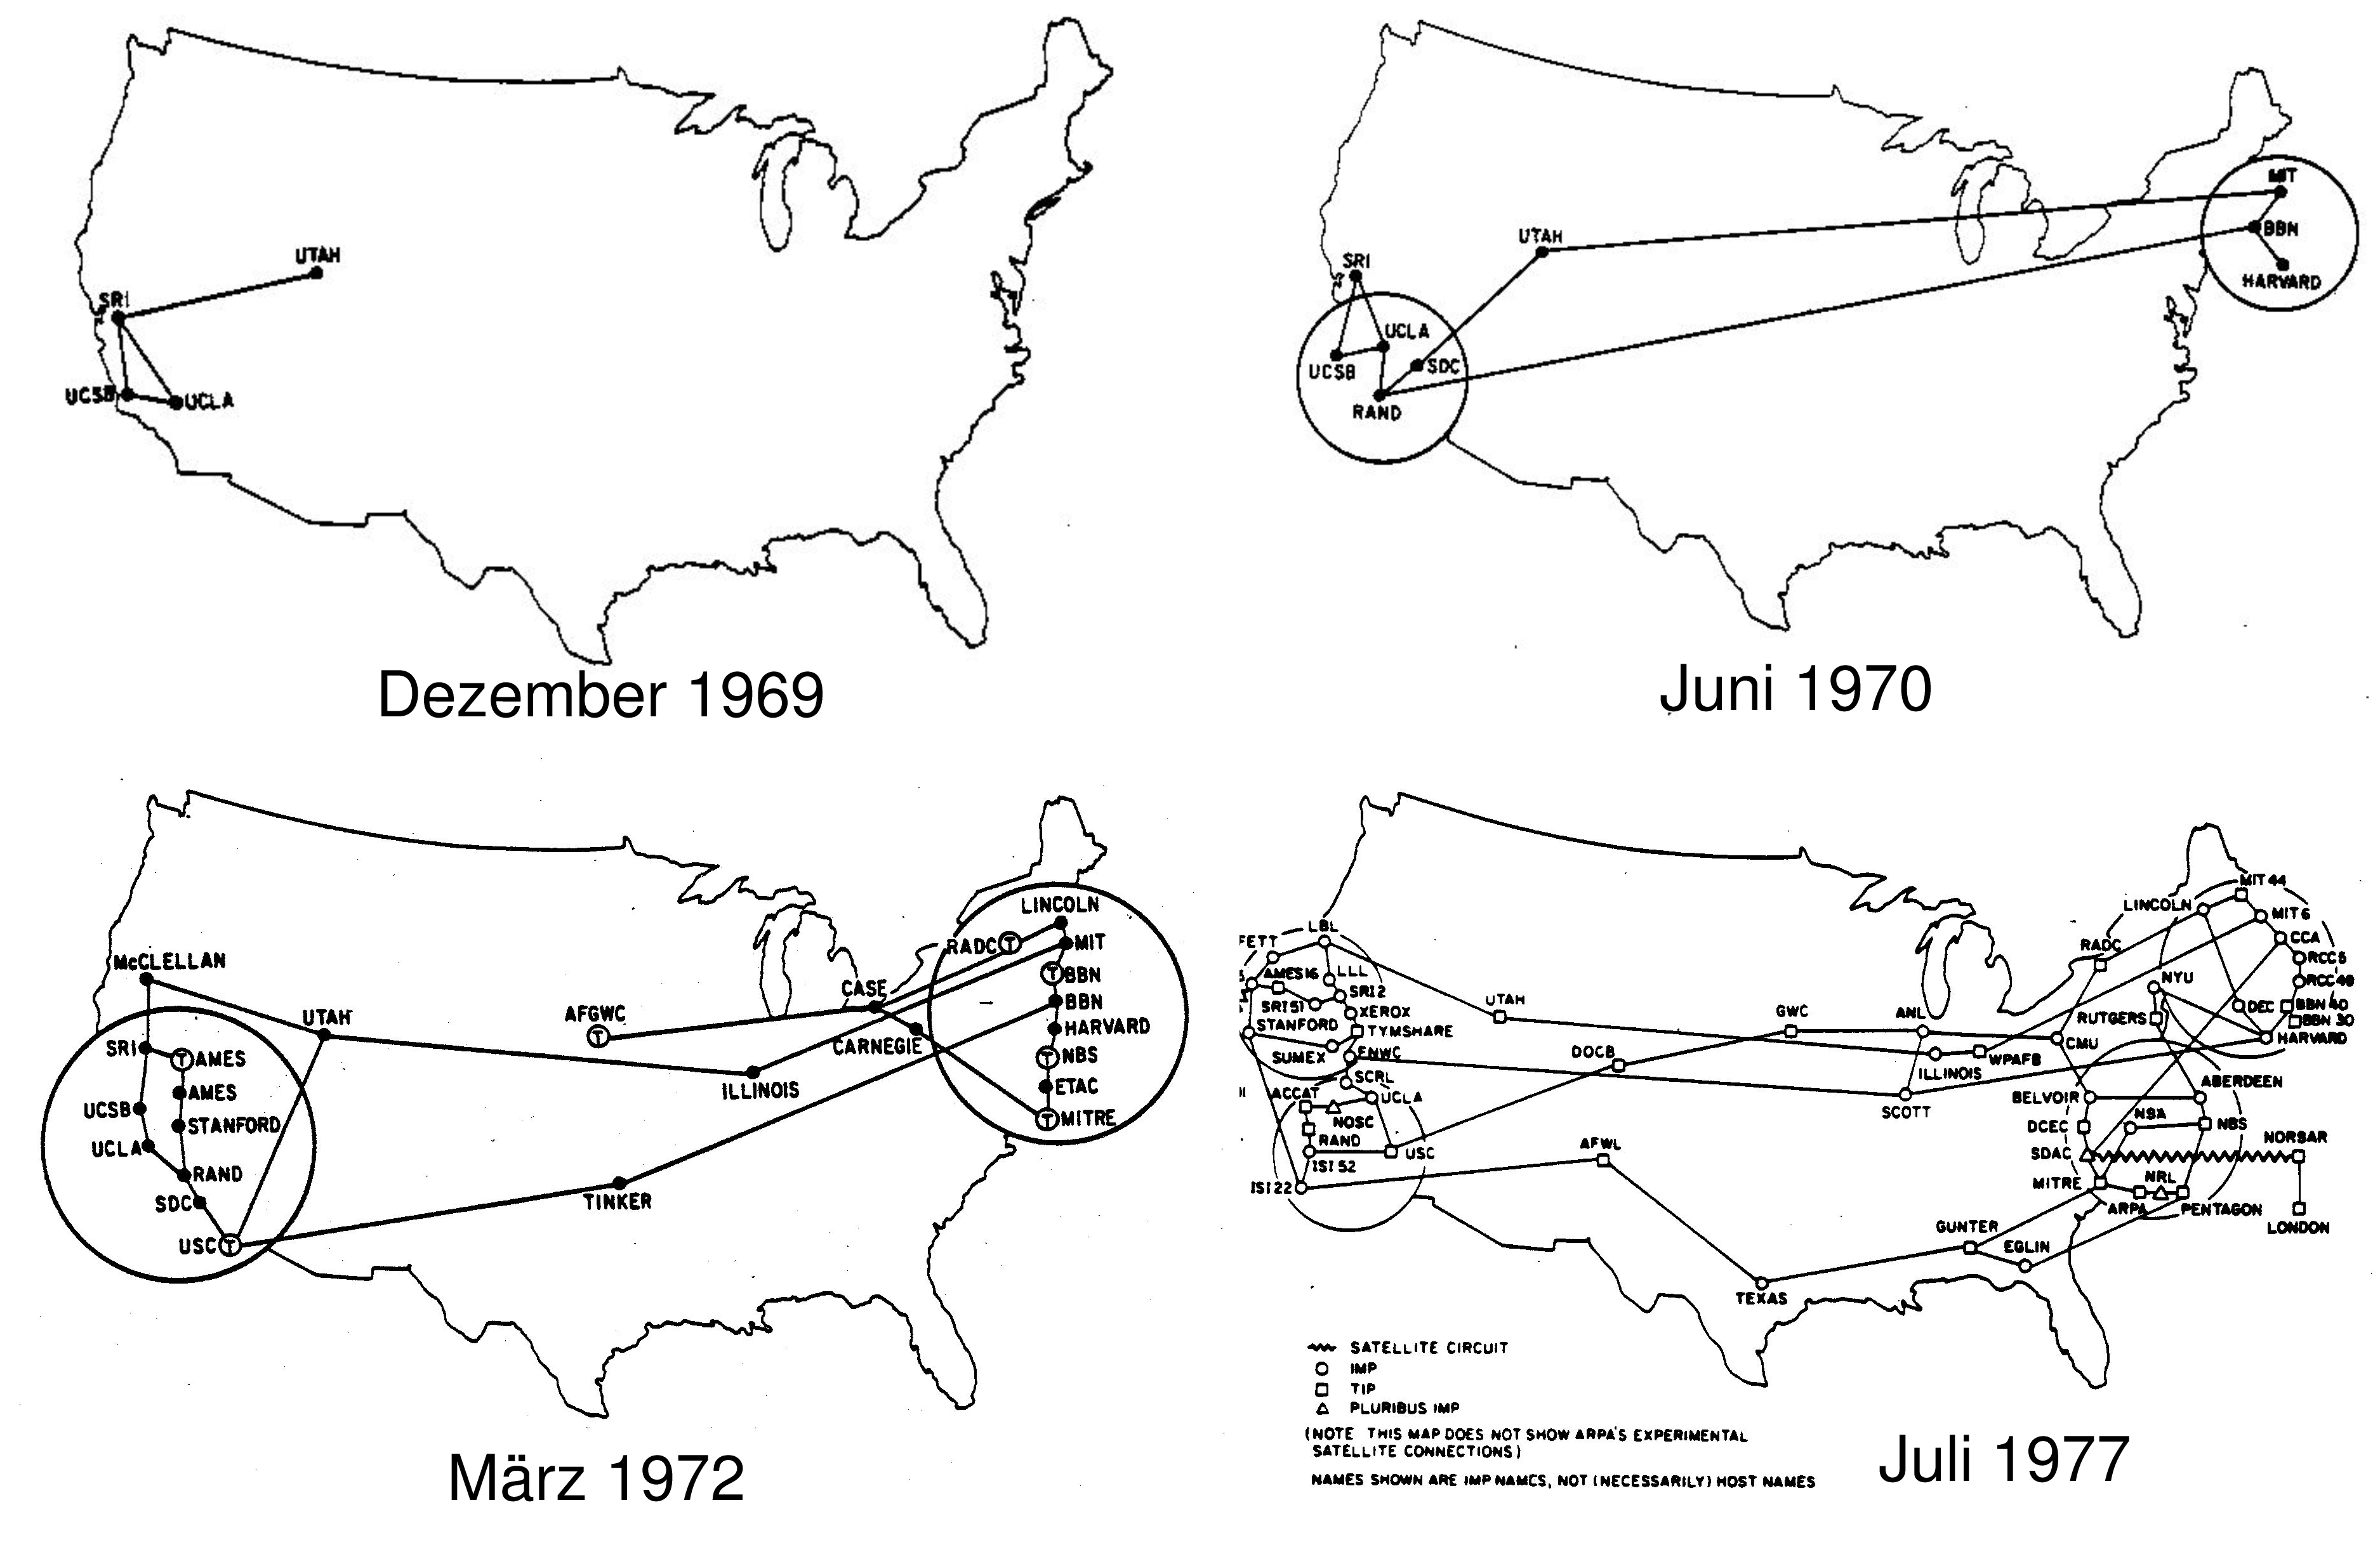
\includegraphics[width=.7\textwidth]{Grundlagen_Info/07_Netzwerke/Figures/arpanet.png}
	\caption{Ausbreitung des \gls{ARPANET} von 1969 bis 1977 (Quelle: \href{http://www.fibel.org/linux/lfo-0.6.0/node457.html}{fibel.org})}
\end{figure}

\subsubsection{Die Entwicklung von Protokollen: \texorpdfstring{\acrshort{TCP}/\acrshort{IP}}{TCP/IP}}
Ein entscheidender Schritt in der Geschichte des Internets war die Entwicklung von Kommunikationsprotokollen, die es verschiedenen Netzwerken ermöglichten, miteinander zu kommunizieren. Insbesondere das \gls{TCP}/\gls{IP}-Protokoll, das 1983 als Standard eingeführt wurde, bildete die Grundlage für das moderne Internet.

\begin{itemize}
	\item 1983: Umstellung des \gls{ARPANET} auf \gls{TCP}/\gls{IP}.
	\item 1980er: Entstehung weiterer Netzwerke (z.B. CSNET, BITNET) und deren Zusammenschluss.
\end{itemize}

Eine schematische Darstellung der Verbindung von verschiedenen Netzwerken über das \gls{TCP}/\gls{IP}-Protokoll ist in \cref{table:osi-layers} zu finden.

\subsubsection*{Das \acrshort{WWW} und die 1990er Jahre}
Die Erfindung des ersten Browsers namens \gls{WWW} durch Tim Berners-Lee im Jahr 1990 revolutionierte die Nutzung des Internets. Kernstück des \gls{WWW} ist das Hypertext Transfer Protocol (\gls{HTTP}), das es ermöglicht, Webseiten zu erstellen und diese gegenseitig zu verlinken. Mit der Einführung von \gls{HTML} konnten Inhalte strukturiert und formatiert werden. Dies führte zu einer explosionsartigen Zunahme von Webseiten und Nutzern. Eine typische Webseite, wie wir sie heute kennen, ist über eine Web-Adresse, oder genauer gesagt \gls{URL} erreichbar, wie in folgendem Beispiel:

\begin{lstlisting}[language=HTML]
https://www.beispielseite.ch/unterseite.html
\end{lstlisting}

Eine \gls{URL} (Uniform Resource Locator) ist eine eindeutige Adresse, die auf eine Ressource (meistens eine Datei) im Internet verweist. Sie besteht aus mehreren Teilen, darunter das Protokoll (\texttt{http://} oder \texttt{https://}), der Domain-Name (\texttt{www.beispielseite.ch}) und der Pfad zur Datei (\texttt{/unterseite.html}).

Der Domain-Name steht für einen Computer im Internet, auf dem die Webseite gespeichert ist. Dieser Computer wird auch als \textbf{Webserver} bezeichnet.

Jede Webseite ist dabei als einfache Textdatei gespeichert, mit der Dateiendung \texttt{.html} (oder \texttt{.htm}). \gls{HTML} ist dabei eine Art Code-Sprache, die es ermöglicht, Text, Bilder und Links zu strukturieren. Eine einfache HTML-Datei könnte zum Beispiel so aussehen:

\begin{lstlisting}[language=HTML]
<!DOCTYPE html>
<html>
<head>
	<title>Beispielseite</title>
</head>
<body>
	<h1>Willkommen auf der Beispielseite</h1>
	<p>Dies ist ein einfacher Textabschnitt.</p>
	<a href="https://www.andereseite.ch/start.html">Andere Webseite</a>
</body>
\end{lstlisting}
Auf der vorletzten Zeile sehen Sie den Link zu einer anderen Webseite. Dieser Link ist ein sogenannter \textbf{Hyperlink}, der es ermöglicht, von einer Webseite zu einer anderen zu navigieren. Hyperlinks sind das Herzstück des \gls{WWW} und ermöglichen die Vernetzung von Informationen im Internet. Sie bestehen aus einem Text (der anklickbar ist) und einer \gls{URL}, die die Adresse der verlinkten Seite angibt. Ein Protokoll namens \gls{HTTP} regelt, wie diese Links angefragt und die entsprechenden Seiten übertragen werden. 

Ein Browser kann den \gls{HTML}-Code benutzerfreundlich anzeigen und Verweise auf andere Webseiten als anklickbare Links anzeigen. Die Kombination von \gls{HTML}, \gls{HTTP} und der \gls{URL} ermöglichte es, Informationen auf einfache Weise zu teilen und zu durchsuchen.

Mit der Einführung von grafischen Webbrowsern wurde das Internet für die breite Öffentlichkeit zugänglich und erlebte einen massiven Popularitätsschub.

\begin{itemize}
	\item 1991: Das \gls{WWW} wird der Öffentlichkeit vorgestellt.
	\item 1993: Der erste grafische Webbrowser (Mosaic) erscheint.
	\item 1995: Kommerzielle Nutzung des Internets wird möglich, Gründung von Unternehmen wie Amazon und eBay.
\end{itemize}

\begin{figure}[H]
	\centering
	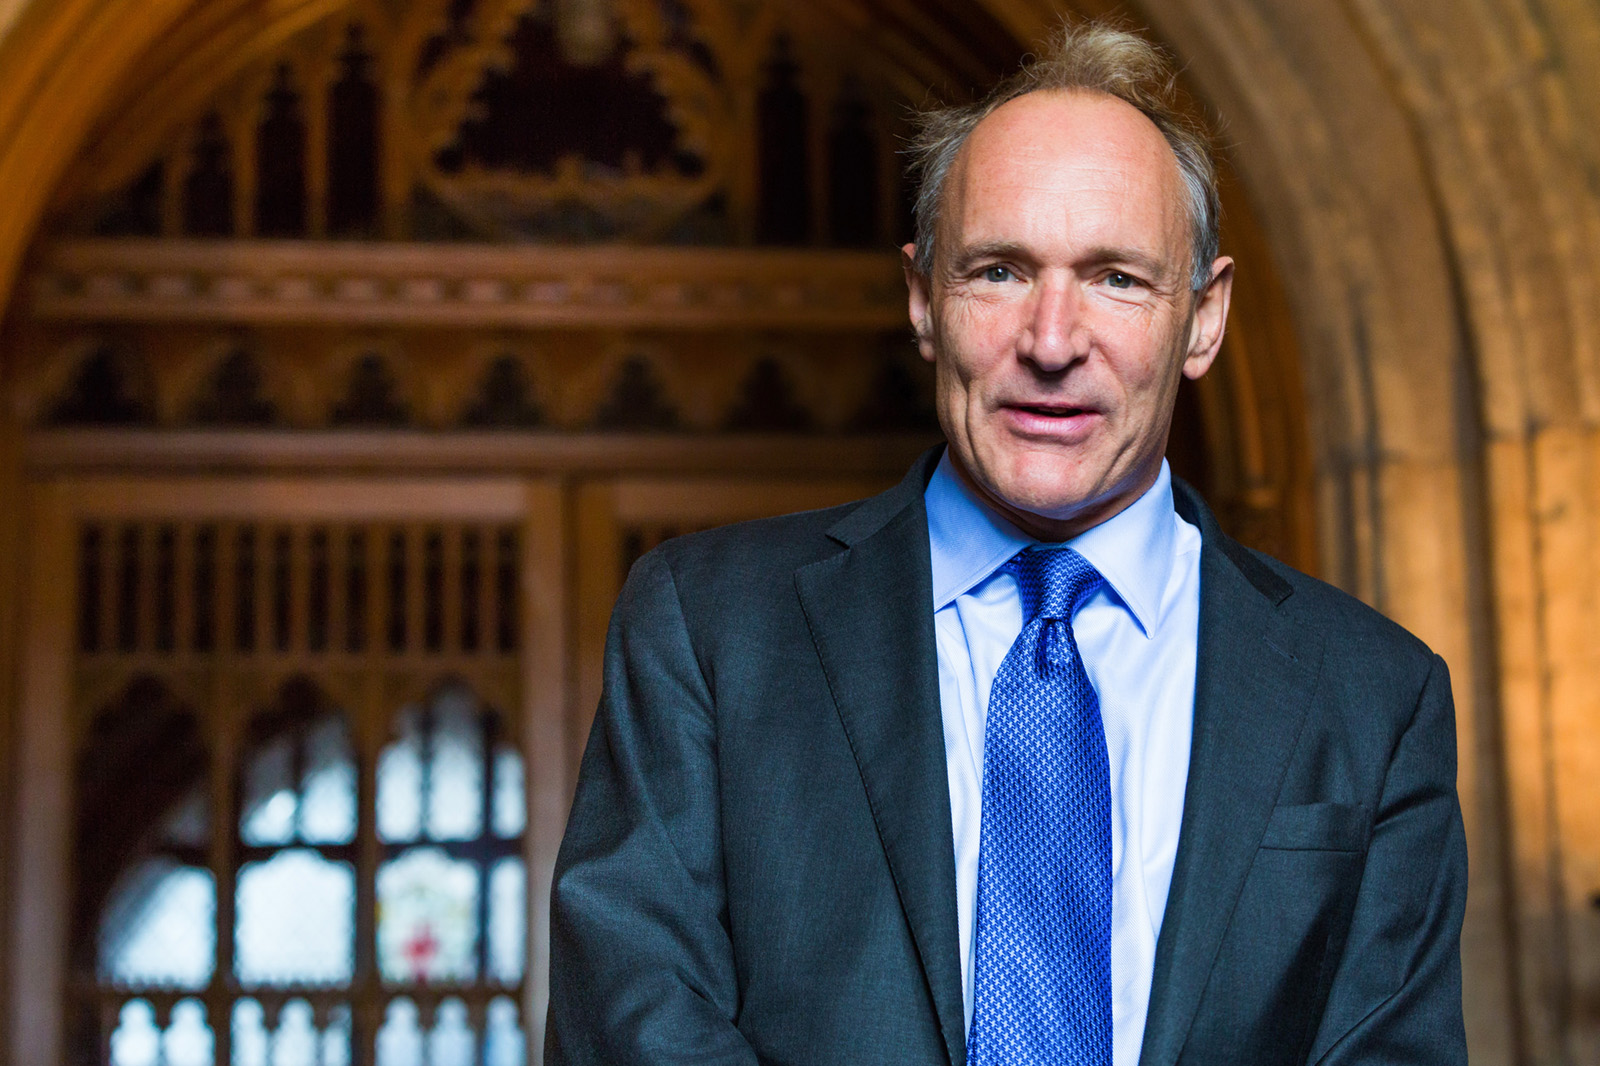
\includegraphics[width=.5\textwidth]{Grundlagen_Info/07_Netzwerke/Figures/tim-berners-lee.jpg}
	\caption{Sir Tim Berners-Lee, der \enquote{Erfinder} des \acrlong{WWW}, 2014 (Quelle: \href{https://de.wikipedia.org/wiki/Tim_Berners-Lee}{Wikipedia})}
\end{figure}

\subsubsection*{Das Internet im 21. Jahrhundert}
Im 21. Jahrhundert hat das Internet weiterhin rasant an Bedeutung gewonnen. Mit der Verbreitung von schnellem Breitband-Internet, Smartphones und sozialen Medien ist das Internet zu einem unverzichtbaren Bestandteil des täglichen Lebens geworden.

Eine der wichtigsten Erfindungen, um das Internet jederzeit und überall verfügbar zu machen, war das \textbf{Mobile Internet}. Mit der Einführung von Smartphones und mobilen Datenverbindungen wurde es möglich, jederzeit auf das Internet zuzugreifen. Dies führte zu einer Explosion von mobilen Anwendungen und Diensten, die das Internet noch zugänglicher machten. Insbesondere die Einführung des iPhones durch die Firma Apple im Jahr 2007 und die damit verbundene Verbreitung von Smartphones haben das Internet revolutioniert. Heute sind Smartphones allgegenwärtig und ermöglichen den Zugriff auf das Internet von nahezu jedem Ort aus.

\begin{itemize}
	\item 2000er: Verbreitung von schnellem Breitband-Internet, Aufstieg von Google, Facebook, YouTube.
	\item 2007: Einführung des iPhones, Beginn der Smartphone-Revolution (s. \href{https://www.youtube.com/watch?v=MnrJzXM7a6o}{Video der Produktvorstellung im Jahr 2007}).
	\item 2010er: Mobile Internetnutzung, Smartphones, \gls{IoT}.
	\item Heute: Künstliche Intelligenz, 5G, weltweite Vernetzung.
\end{itemize}

\begin{figure}[H]
	\centering
	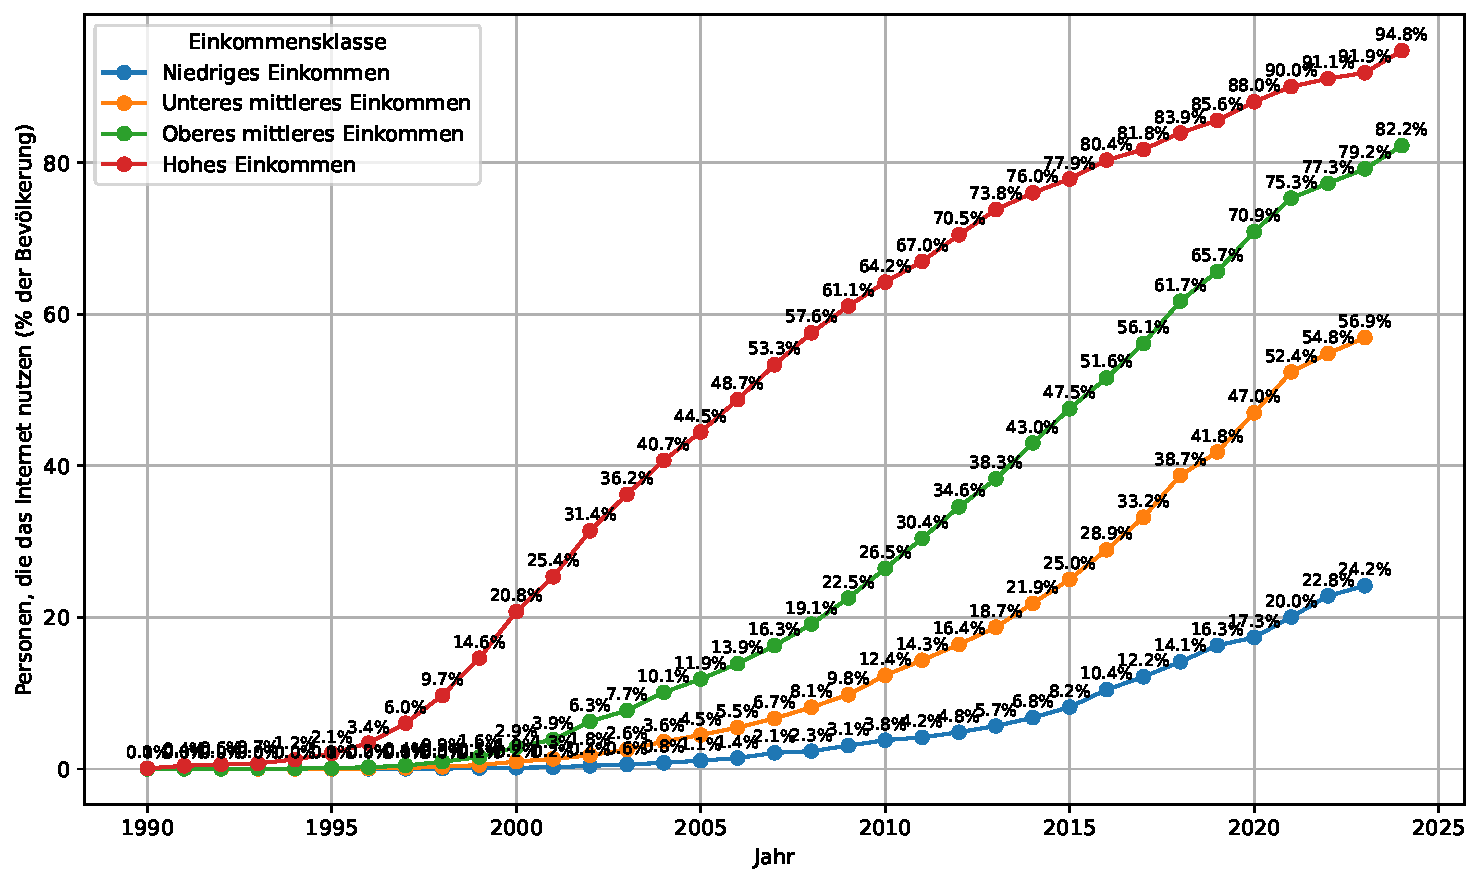
\includegraphics[width=.8\textwidth]{Grundlagen_Info/07_Netzwerke/Figures/internet_use_by_income_class.pdf}
	\caption{Entwicklung der weltweiten Internetnutzung nach Einkommensklasse (Quelle: \href{https://data.worldbank.org/indicator/IT.NET.USER.ZS}{Weltbank-Daten})}
	\label{fig:internet_use_by_income_class}
\end{figure}

Wie auf \cref{fig:internet_use_by_income_class} zu sehen ist, hat sich die Internetnutzung in den letzten Jahren stark erhöht. Insbesondere in einkommensstarken Ländern ist die Internetnutzung nahezu flächendeckend, während in einkommensschwachen Ländern noch grosse Unterschiede bestehen. Dies wird gut ersichtlich auf der Karte (s. \cref{fig:internet_use_by_income_class_map}).

\begin{figure}[H]
	\centering
	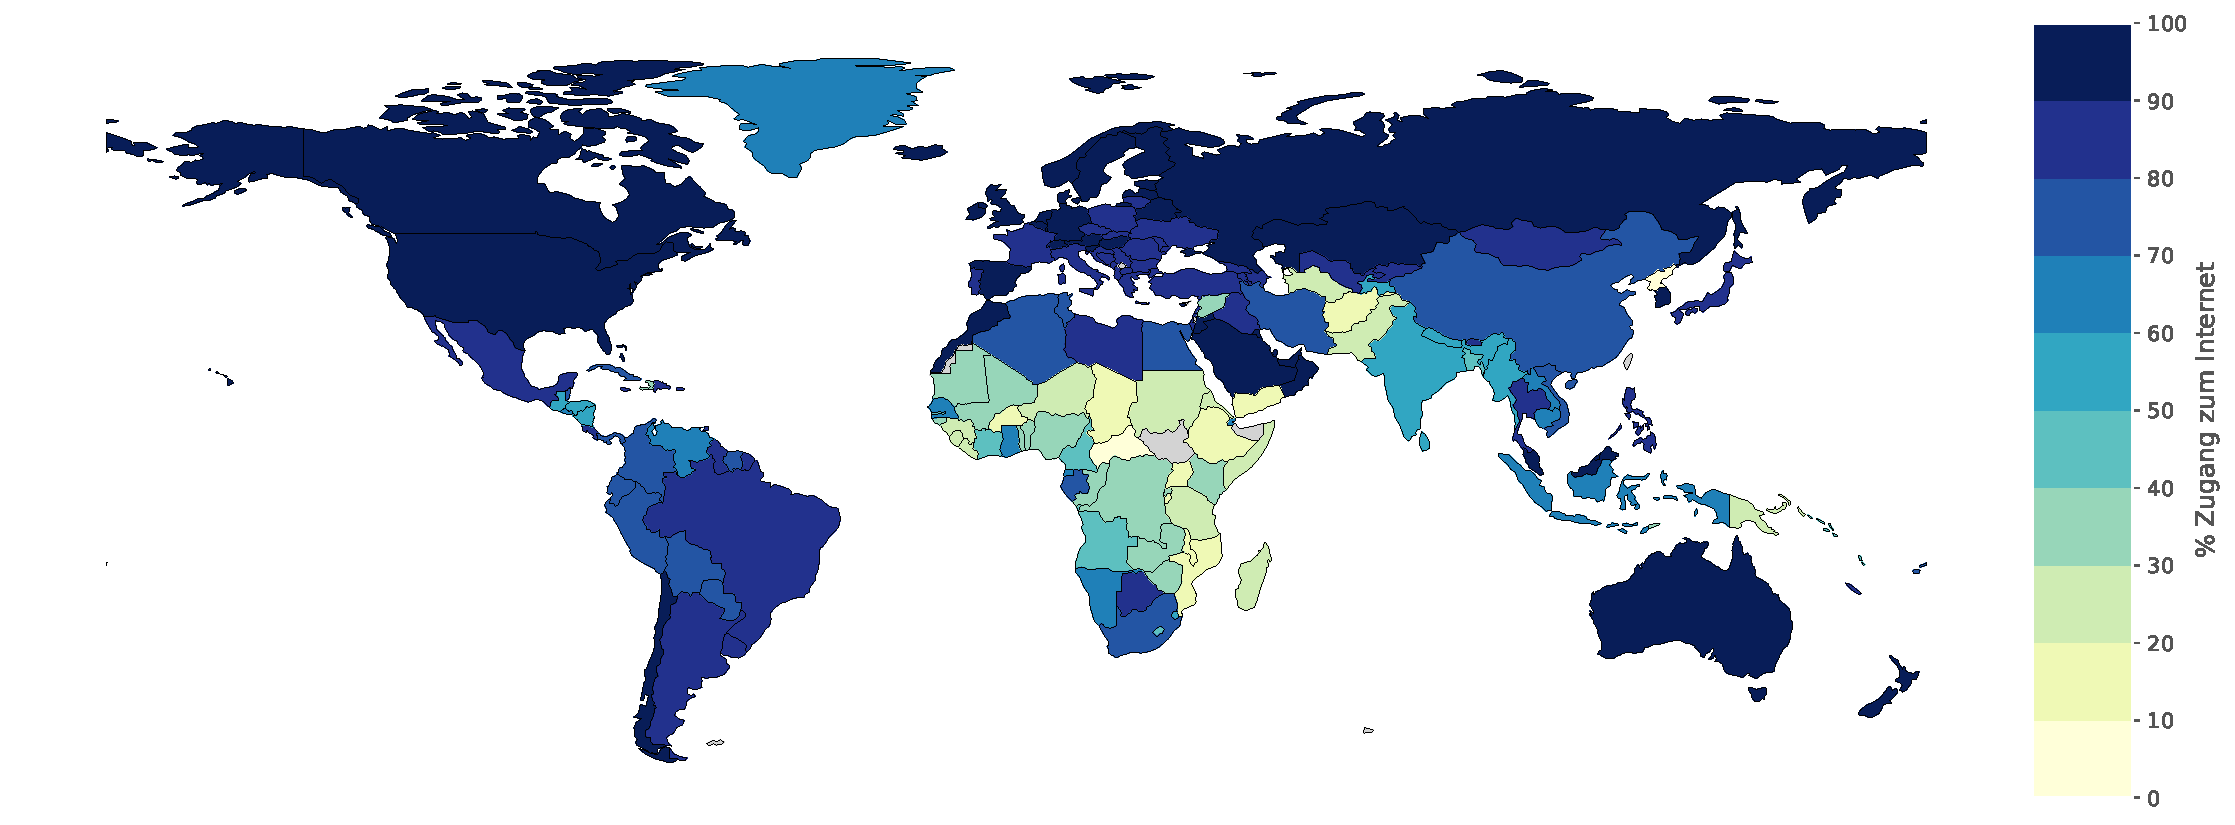
\includegraphics[width=.8\textwidth]{Grundlagen_Info/07_Netzwerke/Figures/internet_use_map_2024.pdf}
	\caption{Internetnutzung nach Land, 2024 (Quelle: \href{https://data.worldbank.org/indicator/IT.NET.USER.ZS}{Weltbank-Daten})}
	\label{fig:internet_use_by_income_class_map}
\end{figure}

\subsection{Topologie}
Beim Erstellen eines Netzwerks stellt sich als Erstes die Frage, welche Computer man mit welchen anderen Computern verbinden soll. Die Struktur der Verbindungen in einem Netzwerk kann also umformuliert werden als Graphen-Problem, bei dem es zu bestimmen gibt, welche Knoten eines Graphen miteinander über eine Kante verbunden werden. Die verschiedenen möglichen Strukturen eines Netzwerks werden auch als \textbf{Topologie} bezeichnet. Einige Beispiel-Topologien sind in \cref{fig:topologie} gezeigt.
\begin{figure}[H]
	\centering
	% Bus Topology
	\begin{subfigure}[b]{0.25\textwidth}
		\centering
		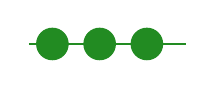
\begin{tikzpicture}
			\draw[ForestGreen, thick] (0,0) -- (2,0); % Bus
			\foreach \x in {0.3, 0.9, 1.5} {
					\filldraw[ForestGreen] (\x, 0) circle (2mm);
				}
		\end{tikzpicture}
		\caption{Bus}
	\end{subfigure}%
	% Ring Topology
	\begin{subfigure}[b]{0.25\textwidth}
		\centering
		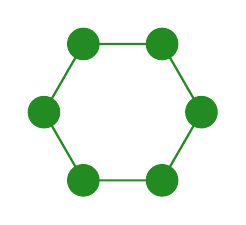
\begin{tikzpicture}
			\draw[ForestGreen, thick] (0:1cm) \foreach \x in {60,120,...,360} {
					-- (\x:1cm)
				} -- cycle; % Completes the circle
			\foreach \x in {0,60,...,300} {
					\filldraw[ForestGreen] (\x:1cm) circle (2mm);
				}
		\end{tikzpicture}
		\caption{Ring}
	\end{subfigure}
	% Stern
	\begin{subfigure}[b]{0.25\textwidth}
		\centering
		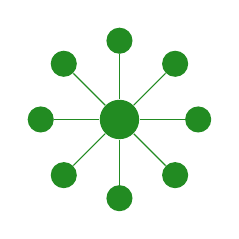
\begin{tikzpicture}
			\node[fill=ForestGreen, circle, minimum size=5mm] at (0,0) (center) {};
			\foreach \x in {0,45,...,315} {
					\node[fill=ForestGreen, circle, minimum size=2mm] at (\x:1cm) (node\x) {};
					\draw[ForestGreen] (center) -- (node\x);
				}
		\end{tikzpicture}
		\caption{Stern}
	\end{subfigure}%
	% Mesh Topology
	\begin{subfigure}[b]{0.25\textwidth}
		\centering
		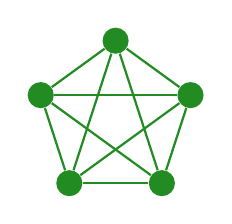
\begin{tikzpicture}
			% Define nodes
			\foreach \x [count=\i from 1] in {18,90,162,234,306} {
					\node[fill=ForestGreen, circle, minimum size=2mm] at (\x:1cm) (node\i) {};
				}

			% Connect nodes (to border points)
			\foreach \x in {1,2,3,4,5} {
					\foreach \y in {\x,...,5} {
							\ifnum\x=\y\relax
								% skip self-connection
							\else
								\draw[ForestGreen, thick] (node\x) -- (node\y);
							\fi
						}
				}

		\end{tikzpicture}
		\caption{Vollvermascht}
	\end{subfigure}
	\begin{subfigure}{.25\textwidth}
		\centering
		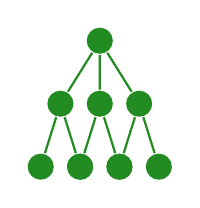
\begin{tikzpicture}[
				sibling distance=5mm, % Adjust spacing between siblings
				level distance=8mm, % Adjust spacing between parent and child nodes
				every node/.style={fill=ForestGreen, circle, thick, minimum size=2mm},
				edge from parent/.style={ForestGreen, thick, draw}
			]
			% Define the tree
			\node {} % Root node
			child {node {}
					child {node {}}
					child {node {}}
				}
			child {node {}
					child {node {}}
					child {node {}}
				}
			child {node {}
					child {node {}}
					child {node {}}
				};

		\end{tikzpicture}
		\caption{Baum}
	\end{subfigure}
	\caption{Beispiele von Netzwerk-Topologien}
	\label{fig:topologie}
\end{figure}

Da Computer in Realität häufig nur über eine einzige Netzwerkkarte verfügen, können sie auch nur mit einem weiteren Computer verbunden werden. In einem lokalen Netzwerk trifft man daher häufig die Form einer Stern-Topologie an, bei der alle Computer mit einer zentralen \textbf{Switch} verbunden werden, also einem Gerät, welches mehrere Rechner an einem zentralen Punkt miteinander verbindet.

\begin{myexercise}
	Vergleichen Sie die Stern-Topologie mit der Vollvermascht-Topologie:
	\begin{itemize}
		\item In welcher Topologie ist es einfacher, ein neues Gerät anzuschliessen?
		\item In welcher Topologie funktioniert die Kommunikation immer noch gut, selbst wenn einzelne Kabel oder Geräte ausfallen?
		\item In welcher Topologie müssen mehr Kabel gekauft werden?
	\end{itemize}
	\begin{myanswer}
		\begin{itemize}
			\item In der Stern-Topologie ist es einfacher, ein neues Gerät anzuschliessen.
			\item In der Vollvermaschten Topologie funktioniert die Kommunikation immer noch gut, selbst wenn einzelne Kabel oder Geräte ausfallen.
			\item In der Vollvermaschten Topologie müssen mehr Kabel gekauft werden.
		\end{itemize}
	\end{myanswer}
\end{myexercise}

\begin{myexercise}
	Wie viele Kabel müssen in der Stern-Topologie gekauft werden\dots
	\begin{itemize}
		\item Für 6 Geräte?
		\item Für 10 Geräte?
		\item Allgemeine Formel?
	\end{itemize}
\begin{myanswer}
	\begin{itemize}
		\item Für 6 Geräte: 5 Kabel
		\item Für 10 Geräte: 9 Kabel
		\item Allgemeine Formel: $n-1$ Kabel, wobei $n$ die Anzahl der Geräte ist.
	\end{itemize}
\end{myanswer}
\end{myexercise}

\begin{myexercise}
	Wie viele Kabel müssen in der Vollvermascht-Topologie gekauft werden\dots
	\begin{itemize}
		\item Für 6 Geräte?
		\item Für 10 Geräte?
		\item Allgemeine Formel?
	\end{itemize}
\begin{myanswer}
	\begin{itemize}
		\item Für 6 Geräte: 15 Kabel
		\item Für 10 Geräte: 45 Kabel
		\item Allgemeine Formel: $\frac{n(n-1)}{2}$ Kabel, wobei $n$ die Anzahl der Geräte ist.
	\end{itemize}
\end{myanswer}
\end{myexercise}

\subsubsection{Unicast, Multicast und Broadcast}
Je nachdem für wie viele Teilnehmer eines Netzwerks eine Sendung bestimmt ist, unterscheidet man bei der Datenübertragung zwischen \textbf{Unicast}, \textbf{Multicast} und \textbf{Broadcast} (s. \cref{fig:unicast-multicast-broadcast}).

\begin{figure}[H]
	\centering
	% Unicast
	\begin{subfigure}[b]{0.3\textwidth}
		\centering
		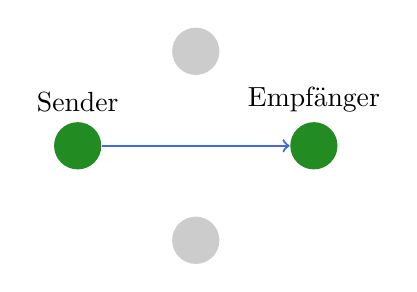
\begin{tikzpicture}
			% Nodes
			\node[fill=ForestGreen, circle, minimum size=6mm, label=above:{Sender}] (A) at (0,0) {};
			\node[fill=ForestGreen, circle, minimum size=6mm, label=above:{Empfänger}] (B) at (3,0) {};
			% Other nodes (not involved)
			\node[fill=Gray!40, circle, minimum size=6mm] (C) at (1.5,1.2) {};
			\node[fill=Gray!40, circle, minimum size=6mm] (D) at (1.5,-1.2) {};
			% Arrows
			\draw[->, thick, RoyalBlue] (A) -- (B);
		\end{tikzpicture}
		\caption{Unicast: 1:1}
	\end{subfigure}%
	% Multicast
	\begin{subfigure}[b]{0.3\textwidth}
		\centering
		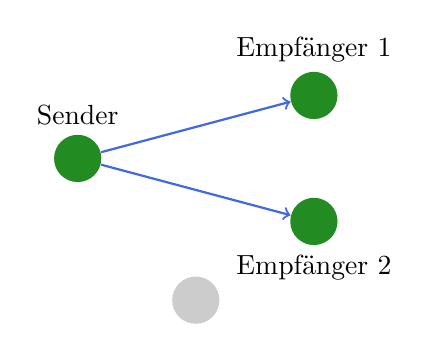
\begin{tikzpicture}
			% Nodes
			\node[fill=ForestGreen, circle, minimum size=6mm, label=above:{Sender}] (A) at (0,0) {};
			\node[fill=ForestGreen, circle, minimum size=6mm, label=above:{Empfänger 1}] (B) at (3,0.8) {};
			\node[fill=ForestGreen, circle, minimum size=6mm, label=below:{Empfänger 2}] (C) at (3,-0.8) {};
			% Other node (not involved)
			\node[fill=Gray!40, circle, minimum size=6mm] (D) at (1.5,-1.8) {};
			% Arrows
			\draw[->, thick, RoyalBlue] (A) -- (B);
			\draw[->, thick, RoyalBlue] (A) -- (C);
		\end{tikzpicture}
		\caption{Multicast: 1:n (Gruppe)}
	\end{subfigure}%
	% Broadcast
	\begin{subfigure}[b]{0.3\textwidth}
		\centering
		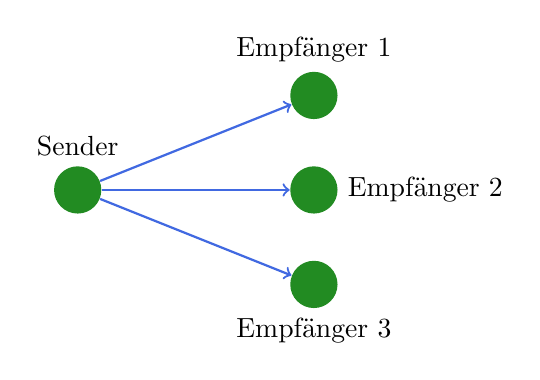
\begin{tikzpicture}
			% Nodes
			\node[fill=ForestGreen, circle, minimum size=6mm, label=above:{Sender}] (A) at (0,0) {};
			\node[fill=ForestGreen, circle, minimum size=6mm, label=above:{Empfänger 1}] (B) at (3,1.2) {};
			\node[fill=ForestGreen, circle, minimum size=6mm, label=right:{Empfänger 2}] (C) at (3,0) {};
			\node[fill=ForestGreen, circle, minimum size=6mm, label=below:{Empfänger 3}] (D) at (3,-1.2) {};
			% Arrows
			\draw[->, thick, RoyalBlue] (A) -- (B);
			\draw[->, thick, RoyalBlue] (A) -- (C);
			\draw[->, thick, RoyalBlue] (A) -- (D);
		\end{tikzpicture}
		\caption{Broadcast: 1:alle}
	\end{subfigure}
	\caption{Unicast, Multicast und Broadcast: Übertragungsarten im Netzwerk}
	\label{fig:unicast-multicast-broadcast}
\end{figure}

\begin{myexercise}
Welche Art der Datenübertragung verwenden die folgenden Alltagssituationen?
\begin{itemize}
	\item Whatsapp-Nachricht an eine befreundete Person
	\item Signalfeuer der chinesischen Mauer
	\item Lautsprecherdurchsage im Flughafen
	\item Lautsprecherdurchsage auf dem Gleis bei der SBB
	\item Shoutbox im Intranet
	\item Frage im Klassenchat
	\item Email-Newsletter der Schulleitung
\end{itemize}
\begin{myanswer}
\begin{itemize}
	\item Whatsapp-Nachricht an eine befreundete Person: \textbf{Unicast} (1:1)
	\item Signalfeuer der chinesischen Mauer: \textbf{Multicast oder Broadcast} (an mehrere Wachtürme, aber nicht an alle Menschen in der Umgebung)
	\item Lautsprecherdurchsage im Flughafen: \textbf{Broadcast} (an alle Anwesenden)
	\item Lautsprecherdurchsage auf dem Gleis bei der SBB: \textbf{Multicast} (an alle auf dem Gleis aber nicht an alle Anwesenden im Bahnhof)
	\item Shoutbox im Intranet: \textbf{Broadcast} (an alle Nutzer der Shoutbox)
	\item Frage im Klassenchat: \textbf{Multicast} (an eine bestimmte Gruppe, z.B. die Klasse)
	\item Email-Newsletter der Schulleitung: \textbf{Multicast} (an eine definierte Empfängergruppe)
\end{itemize}
\end{myanswer}
\end{myexercise}

\newpage
\section{Internet-Schichten}
\subsection{Schichtenmodell: Analogie}
Die Kommunikation über das Internet verläuft in unterschiedlichen Teilschritten. Man spricht von dem \textit{Schichtenmodell}. Als Analogie zum Schichtenmodell sei folgende Situation gegeben, in der die Chefs zweier unterschiedlicher Firmen miteinander kommunizieren wollen (siehe \cref{fig:schichtenmodellAnalogie}):
\begin{enumerate}
	\item Chef 1 (\faFemale, in Europa) möchte mit Chef 2 (\faMale, in Asien) sprechen.
	\item Dazu übermittelt Chef 1 dem Sekretariat Ihre Nachricht an Chef 2. Das Sekretariat schreibt die Nachricht nieder und übermittelt der lokalen Post den Brief an Chef 2.
	\item Die lokale Post kümmert sich nun um den Transport zur asiatischen Post, wo der Brief an das Sekretariat von Firma 2 übergeben und schlussendlich an Chef 2 gelangt.
\end{enumerate}

\begin{figure}[H]
	\centering
	\begin{tikzpicture}[
			auto,
			block/.style={
					minimum width=3cm,
					node distance=1.5cm,
					rectangle,
					fill=RoyalBlue!50,
					align=center,
					rounded corners
				}
		]


		% Define the nodes with FontAwesome icons
		\node[block] (chefs) {\faFemale\ Chef};
		\node[block, below=of chefs] (secretariat) {\faPhone\ Sekretariat};
		\node[block, below=of secretariat] (postman) {\faMale\ Post};


		% Define the nodes with FontAwesome icons

		\node[block, right=of postman] (postman2) {\faMale\ Post};
		\node[block, above=of postman2] (secretariat2) {\faPhone\ Sekretariat};
		\node[block, above=of secretariat2] (chefs2) {\faMale\ Chef};


		% Draw the dashed arrows
		\draw[<->, dashed, RoyalBlue!50, thick] (chefs) -- (chefs2);
		\draw[<->, dashed, RoyalBlue!50, thick] (secretariat) -- (secretariat2);
		\draw[<->, dashed, RoyalBlue!50, thick] (postman) -- (postman2);

		\draw[->, line width=1mm,ForestGreen!50] (chefs) -- node[left]{\faComments} (secretariat) ;
		\draw[->, line width=1mm,ForestGreen!50] (secretariat) -- node[left]{\faEnvelope} (postman) ;
		\draw[->, line width=1mm,ForestGreen!50, bend right] (postman.south) to node[midway,below]{\faBicycle\ \faMotorcycle\ \faCar\ \faShip\ \faPlane} (postman2.south) ;
		\draw[->, line width=1mm,ForestGreen!50] (postman2) -- node[right]{\faEnvelope} (secretariat2) ;
		\draw[->, line width=1mm,ForestGreen!50] (secretariat2) -- node[right]{\faComments} (chefs2) ;

		% fit rectangles around regions
		\node[fit=(chefs) (postman), inner sep=8pt, red, dotted, draw, line width=1pt,rounded corners](region1) {};
		\node[fit=(chefs2) (postman2), inner sep=8pt, red, dotted, draw, line width=1pt,rounded corners](region2) {};
		% annotate both rectangles
		\node[above=5pt of region1.north, anchor=center, align=center]{\textcolor{red}{Firma 1, Europa}};
		\node[above=5pt of region2.north, anchor=center, align=center]{\textcolor{red}{Firma 2, Asien}};

	\end{tikzpicture}
	\label{fig:schichtenmodellAnalogie}
	\caption{Analogie zum Schichtenmodell: Kommunikation zwischen zwei grossen Firmen}
\end{figure}

Dieser Kommunikationsablauf kann in Schichten mit jeweiligen dazugehörigen Prozessen aufgeteilt werden:
\begin{enumerate}
	\item \textbf{Schicht ``Chefs''}: damit die beiden Chefs mit einander sinnvolle Gespräche führen können, verfügen Sie über gemeinsame Standards (Sprache, Wissen etc.) sowie Protokolle (standardisierte Abläufe der Begrüssung etc.).
	\item \textbf{Schicht ``Sekretariat''}: Damit die Sekretariate miteinander kommunizieren können, benötigen auch sie standardisierte Abläufe oder Protokolle, etwa, wie man einen Brief korrekt verfässt, datiert und addressiert.
	\item \textbf{Schicht ``Post''}: Die Post verfügt ebenfalls über standardisierte Protokolle (wie werden Briefe und Pakete von A nach B transportiert? Mit welchen Transportmitteln, über welche Routen?)
\end{enumerate}
Die Vorteile des Schichtenmodells scheinen offensichtlich:
\begin{itemize}
	\item \textbf{Unabhängigkeit der Schichten}: Falls die Post das Transportmittel ändert, müssen die Sekretariate die Briefe nicht neu verfassen.
	\item \textbf{Modularität und Spezialisierung}: Statt das jemand alles tun muss (Chef 1 reist nach Asien zu Chef 2), kann der Prozess für die jeweiligten Beteiligten schnell und effizient abgewickelt werden.
\end{itemize}

\subsection{TCP-IP- und OSI-Schichtenmodell}

Im Zusammenhang mit dem Internet werden häufig zwei Schichtenmodelle gegenübergestellt: Das vollständige, detaillierte \acrfull{OSI}-Modell mit 7 Schichten sowie das etwas vereinfachte \acrfull{TCP}-\acrfull{IP}-Modell mit 4 Schichten. Die beiden Schichten, deren Aufgaben, Informationsformen und Protokolle sind in \cref{table:osi-layers} abgebildet.


\begin{table}[H]
	\centering
	\footnotesize
	\begin{tabular}{c|m{2.6cm}||m{2cm}||m{4.6cm}|m{2.5cm}|m{2cm}}
		\textbf{\#}              & \textbf{Schicht (OSI)}                     & \textbf{Schicht \newline (TCP / IP)}  & \textbf{Aufgabe}                                                                                                & \textbf{Informations\-form}       & \textbf{Gerät / \newline Protokoll}   \\ \midrule\midrule
		\rowcolor{yellow!10}7    & Anwendung \newline \textit{Application}    & Anwendung\newline\textit{Application} & Hilft bei der Identifizierung des Clients und synchronisiert die Kommunikation.                                 & Nachricht                                 & \textbf{HTTP(S)}, FTP, SMTP...        \\\midrule
		\rowcolor{yellow!20}6    & Darstellung \newline \textit{Presentation} & Anwendung\newline\textit{Application} & Daten von der Anwendungsschicht werden extrahiert und für die Übertragung in das erforderliche Format gebracht. & Nachricht                                 & JPEG, MPEG, GIF, \textbf{HTML}...     \\\midrule
		\rowcolor{yellow!30}5    & Sitzung \newline \textit{Session}          & Anwendung\newline\textit{Application} & Stellt Verbindung her, hält diese aufrecht, gewährleistet Authentifizierung und sichert die Sicherheit.         & Nachricht (oder verschlüsselte Nachricht) & Gateway, NetBIOS, PPTP, ...           \\\midrule
		\rowcolor{orange!20}4    & Transport\newline \textit{Transport}       & Transport\newline\textit{Transport}   & Nimmt Dienst von der Vermittlungsschicht und stellt ihn der Anwendungsschicht zur Verfügung.                    & Segment                                   & Firewall, \textbf{TCP}, UDP, Ports... \\\midrule
		\rowcolor{RoyalBlue!20}3 & Vermittlung \newline \textit{Network}      & Internet\newline\textit{Internet}     & Übertragung von Daten von einem Host zu einem anderen, der sich in unterschiedlichen Netzwerken befindet.       & Paket                                     & Router, \textbf{IPv4}, IPv6           \\\midrule
		\rowcolor{Gray!15}2      & Sicherung \newline \textit{Data Link}      & Netzzugriff\newline\textit{Data Link} & Übermittlung von Nachrichten von Knoten zu Knoten.                                                              & Frame                                     & Switch, Bridge, \textbf{MAC}...       \\\midrule
		\rowcolor{Gray!25}1      & Bitübertragung \newline \textit{Physical}  & Netzzugriff\newline\textit{Data Link} & Herstellung physischer Verbindungen zwischen Geräten.                                                           & Bits                                      & Hub, Repeater, Modem, Kabel...        \\
	\end{tabular}
	\label{table:osi-layers}
	\caption{Internet-Schichten-Modelle \gls{OSI} und \gls{TCP}-\gls{IP} sowie deren wichtigste Aufgaben, Informationsformen, Geräte und Protokolle}
\end{table}

Im Folgenden gehen verwenden wir hauptsächlich das etwas vereinfachte \acrfull{TCP}-\acrfull{IP}-Modelle und gehen kurz auf jede Schicht ein.



\begin{myexercise}
	Um sich auf die Vertiefung in die jeweiligen Schichten und Protokolle einzustimmen, schauen Sie sich folgendes Video an:

	\begin{figure}[H]
		\href{https://www.youtube.com/watch?v=PBWhzz_Gn10}{Youtube-Video (13')}
	\end{figure}

	Notieren Sie sich dabei Ihre Antworten auf folgende Fragen:
	\begin{itemize}
		\item Welche \textbf{Schichten}, \textbf{Geräte} und \textbf{Protokolle} werden genannt?
		      \begin{itemize}
			      \item Namen (Abkürzung und ganz)
			      \item Wofür sind sie zuständig?
			      \item Welche Protokolle gehören zu welchen Schichten?
			      \item Welche Geräte gehören zu welchen Protokollen / Schichten?
		      \end{itemize}
		\item Notieren Sie Ihre \textbf{Fragen}: Welche Begriffe verstehen Sie (noch) nicht?
	\end{itemize}

\end{myexercise}

\begin{myexercise}
	Tauschen Sie sich nun in 3er- bis 4er-Gruppen aus und tragen Sie ihre Notizen zusammen. Beantworten Sie danach folgende Fragen:
	\begin{itemize}
		\item Was ist eine URL?
		\item Was macht ``Mr. IP''?
		\item Was macht der Router?
		\item Was macht die Firewall?
		\item Was macht der Proxy Server?
		\item Was macht der ``Ping of Death''? \faSkull
	\end{itemize}
\end{myexercise}

\subsection{Anwendungsschicht}

Bevor wir uns näher mit den Dimensionen der Anwendungsschicht sowie der darunterliegenden Schichten befassen, sollten wir zuerst einige häufig auftauchende Begriffe klären, von denen im Kontext von Rechner-Netzen häufig die Rede ist. Je nach Rolle der Computer in einem Rechner-Netz ist häufig von \textbf{Client}, \textbf{Server} oder \textbf{Host} die Rede:
\begin{itemize}
	\item Der \textbf{Client} $\mathcal{C}$ (von en. \textit{client} = ``Kunde'') bezeichnet den Computer $\mathcal{C}$, der etwas von einem anderen Computer $\mathcal{S}$ will. Genauer gesagt handelt es sich nicht um den Computer selber, sondern um ein Programm auf einem Computer $\mathcal{C}$, das etwas anfordert von einem anderen Programm, das auf einem anderen Computer $\mathcal{S}$ läuft. Zur Vereinfachung sprechen wir jedoch häufig einfach von einem Computer $\mathcal{C}$ und einem Computer $\mathcal{S}$.
	\item Der \textbf{Server} $\mathcal{S}$ (von en. \textit{to serve} = ``dienen'') bezeichnet  den Computer $\mathcal{S}$ (genauer gesagt das Computer-Programm $\mathcal{S}$), das dem Computer $\mathcal{C}$ gibt, was er will. Der Server kann Verbindungsanfragen von anderen Computern akzeptieren oder ablehnen.
	\item Bei einem \textbf{Host} (von englisch \textit{host} = ``Wirt'' / ``Gastgeber'') ist im allgemeinen ein Computer in einem Netzwerk gemeint, der je nach Situation die Rolle des Servers oder Clients einnehmen kann. Der Name eines Computers in einem Netzwerk wird häufig als \textbf{Host Name} bezeichnet.
\end{itemize}

\subsection{Transportschicht}
In der Transportschicht geht es, wie es der Name bereits sagt, darum, wie Daten von einem Host zum nächsten transportiert werden.

Die Daten, die zwischen zwei Computern übertragen werden, werden häufig auch als \textbf{Nutzdaten} oder \textit{payload} bezeichnet. Zu diesen Nutzdaten, die zwischen zwei Computern hin- und hergesandt werden sollen, kommen nun noch verschiedene weitere Daten dazu, so genannte \textbf{Metadaten}. Metadaten sind dazu zuständig, wichtige Informationen zu den Ursprungsdaten hinzuzufügen, in diesem Falle Daten, um den Transport der Daten zu ermöglichen. Diese Metadaten werden vom Übertragungs-Steuerungs-Protocoll (\gls{TCP}) zur Verfügung gestellt und genutzt, in einem so genannten \textit{Header} (s. \cref{fig:tcp-header}).

\begin{figure}[H]
	\centering
	\begin{tabular}{>{\raggedright\arraybackslash}p{4cm}|>{\raggedright\arraybackslash}p{4cm}}

		\rowcolor{orange!20}\multicolumn{2}{c}{\textbf{TCP Header}} \\ \midrule\midrule
		Source Port & Destination Port                              \\ \midrule
		\multicolumn{2}{c}{Sequence \# (SEQ)}                       \\ \midrule
		\multicolumn{2}{c}{Acknoledgement \# (ACK)}                 \\ \midrule
		\multicolumn{2}{c}{Weitere TCP-Header-Felder}               \\ \midrule
		\rowcolor{orange!20}\multicolumn{2}{c}{\textbf{Nutzdaten}}  \\ \midrule\midrule
		\multicolumn{2}{c}{Anwendungsdaten}                         \\
	\end{tabular}
	\caption{\gls{TCP}-Header (vereinfachte Darstellung)}
	\label{fig:tcp-header}
\end{figure}


Einige der wichtigsten Metadaten sind:

\begin{itemize}
	\item \textbf{Der Port} (von engl. \textit{port} = Hafen): Dies ist eine Zahl, mit der der Computer weiss, welche Anwendung (z.B. Mail, Browser, Gaming-Programm etc.) Daten verschickt. Ein Computer kann, wie Sie vermutlich wissen, gleichzeitig über mehrere Programme Daten von anderen Computern empfangen und an sie schicken: sie können beispielsweise gleichzeitig eine Nachricht über WhatsApp schicken und ein Video schauen. Damit der Computer weiss, welche Anwendung die Daten verschickt, verseht er die Daten typischerweise mit einem Port. Obschon Ports für jedes Programm frei gewählt werden können, werden für bekannte Protokolle typischerweise Standard-Portnummern verwendet (s. \cref{tab:tcpPorts}).
	      \begin{table}[H]
		      \centering
		      \begin{tabular}{c||c|c}
			      \toprule
			      \textbf{Port} & \textbf{Anwendung} & \textbf{Verwendung}                   \\
			      \midrule
			      20            & \acrfull{FTP}      & Dateitransfer                         \\
			      21            & \acrfull{FTP}      & Befehlssteuerung                      \\
			      22            & \acrfull{SSH}      & Sichere Shell-Zugriffe                \\
			      23            & Telnet             & Unverschlüsselte Fernsteuerung        \\
			      25            & \acrfull{SMTP}     & E-Mail-Versand                        \\
			      53            & \acrfull{DNS}      & Namensauflösung                       \\
			      80            & \acrfull{HTTP}     & Webseiten-Abruf                       \\
			      110           & \acrfull{POP3}     & E-Mail-Abholung                       \\
			      143           & \acrfull{IMAP}     & E-Mail-Management                     \\
			      443           & \acrfull{HTTPS}    & Verschlüsselter Webseiten-Abruf       \\
			      993           & \acrfull{IMAP}     & E-Mail-Management über \acrshort{SSL} \\
			      995           & \acrfull{POP3}     & E-Mail-Abholung über \acrshort{SSL}   \\
			      \bottomrule
		      \end{tabular}
		      \caption{Gängige \gls{TCP}-Ports, Anwendungen und deren Verwendung}
		      \label{tab:tcpPorts}
	      \end{table}
	      Sowohl der \textit{Client} wie auch der \textit{Server} versehen die Daten mit jeweils einer Zahl, die für den Ursprungs-Port (\textit{Source Port}), respektive den Ziel-Port (\textit{Destination Port}) stehen.
	\item \textbf{Ziffern} für die \textit{Sequence} (Sequenz) und \textit{Acknowledgement} (Anerkennung) von Paketen, die die richtige Reihenfolge der gesendeten und erhaltenen Daten gerantieren.
	\item Weitere Daten, die für den Transport notwendig sind.
\end{itemize}

\begin{mychallenge}
	Lösen Sie die Socket- und Port-Aufgaben auf folgendem Link: \url{https://www.inf-schule.de/rechnernetze/anwendung/socketprogrammierung/Anfragen_an_einen_Server_Stellen}.
\end{mychallenge}

Zusätzlich zur Steuerung der Datenübertragung können \gls{TCP}-Metadaten genutzt werden, um die erste Verbindung zwischen zwei Computern herzustellen. Dies erfolgt typischerweise über das 3-Wege-Handschlag-Protokoll (s. \cref{fig:threewayHandshake}).

\begin{figure}[H]
	\centering
	\begin{tikzpicture}[>=Stealth, node distance=4cm and 8cm]
		% Draw the entities
		\tikzset{c/.append style={fill=RoyalBlue!30,rounded corners, align=center, text width=5cm}}
		\tikzset{person/.append style={text width=2.5cm,fill=ForestGreen!30,rounded corners,align=center}}
		\node[person](Bob) {\faMale{} Bob\\\texttt{10.0.0.2:21}};
		\node[person, right=of Bob] (Alice) {\faFemale{} Alice\\\texttt{10.0.0.3:21}};
		% Draw the arrows and labels
		\draw[->, thick, red, dashed] (Bob.south) -- node[c] { Ich möchte mit dir sprechen, Alice, auf Port 21. Bist du offen?\\SYN=1, SEQ\# 10} ([yshift=-3cm]Alice.south);
		\draw[->, thick, red, dashed] ([yshift=-3cm]Alice.south) -- node[c] { Ok, lass uns reden Bob! Ich bin offen auf Port 21.\\SYN=1, ACK=1, ACK=11} ([yshift=-6cm]Bob.south);
		\draw[->, thick, red, dashed] ([yshift=-6cm]Bob.south) -- node[c] { Ok, danke Alice.\\ACK=1, SEQ\#11} ([yshift=-9cm]Alice.south);

		\node[below of=Bob, yshift=-7cm] (BobZeit) {Zeit};
		\node[below of=Alice, yshift=-7cm] (AliceZeit) {Zeit};

		% Time line
		\draw[->, thick] (Bob.south) -- node[xshift=-.2cm, rotate=270] {Zeitachse von Bob} (BobZeit);
		\draw[->, thick] (Alice.south) -- node[xshift=.2cm, rotate=270] {Zeitachse von Alice} (AliceZeit);
	\end{tikzpicture}
	\caption{Drei-Wege-Handschlag im \gls{TCP}-Protokoll}
	\label{fig:threewayHandshake}
\end{figure}
Folgende Schritte des Drei-Wege-Handschlags werden in \cref{fig:threewayHandshake} illustriert:
\begin{enumerate}
	\item Computer A (\textit{client}, \texttt{10.0.0.2}) erstellt eine Verbindungsanfrage zum Computer B (\textit{server}, \texttt{10.0.0.3}), mittels einem Paket, das nur das \texttt{SYN}-Flaggen gesetzt hat.
	\item Der Server antwortet sowohl mit einem gesetzten \texttt{SYN} und einem \texttt{ACK}-Flaggen
	\item Im letzten Schritt antwortet der \textit{client} nochmals mit einem einzelnen \texttt{ACK}-Flaggen\\
\end{enumerate}
Somit ist die \gls{TCP}-Verbindung ist nun erstellt und die beiden Maschinen können miteinander kommunizieren.

\begin{myexercise}[Fragen zum Drei-Wege-Handschlag \cite{InfSchuleVerbindungsaufbau}]
	Erklären Sie, weshalb es in folgendem Beispiel nicht sinnvoll wäre, dass Bob morgen ins Kino ginge.
	\begin{figure}[H]
	\centering
	\begin{tikzpicture}[>=Stealth, node distance=4cm and 8cm]
		% Draw the entities
		\tikzset{c/.append style={fill=RoyalBlue!30,rounded corners, align=center, text width=5cm}}
		\tikzset{person/.append style={text width=2.5cm,fill=ForestGreen!30,rounded corners,align=center}}
		\node[person](Bob) {\faMale{} Bob\\\texttt{10.0.0.2:21}};
		\node[person, right=of Bob] (Alice) {\faFemale{} Alice\\\texttt{10.0.0.3:21}};
		
		% Draw the arrows and labels
		\draw[->, thick, red, dashed] (Bob.south) -- node[c] { Treffen wir uns morgen um 20:00 im Kino?\\SYN=1, SEQ\# 10} ([yshift=-3cm]Alice.south);
		% \draw[->, thick, red, dashed] ([yshift=-3cm]Alice.south) -- node[c] { Ok, lass uns reden Bob! Ich bin offen auf Port 21.\\SYN=1, ACK=1, ACK=11} ([yshift=-6cm]Bob.south);
		% \draw[->, thick, red, dashed] ([yshift=-6cm]Bob.south) -- node[c] { Ok, danke Alice.\\ACK=1, SEQ\#11} ([yshift=-9cm]Alice.south);

		\node[below of=Bob, yshift=-1cm] (BobZeit) {Zeit};
		\node[below of=Alice, yshift=-1cm] (AliceZeit) {Zeit};

		% Time line
		\draw[->, thick] (Bob.south) -- node[xshift=-.2cm, rotate=270] {Zeitachse von Bob} (BobZeit);
		\draw[->, thick] (Alice.south) -- node[xshift=.2cm, rotate=270] {Zeitachse von Alice} (AliceZeit);
	\end{tikzpicture}
	\label{fig:threewayHandshakeEx1}
\end{figure}
\begin{myanswer}
	Bob sollte nicht einfach ins Kino gehen, weil er keine Bestätigung von Alice erhalten hat. Im Drei-Wege-Handschlag muss der Empfänger (Alice) die Anfrage bestätigen, bevor eine Verbindung (bzw. ein Treffen) zustande kommt. Ohne Antwort weiss Bob nicht, ob Alice die Nachricht erhalten hat oder überhaupt kommen wird.
\end{myanswer}
\end{myexercise}

\begin{myexercise}[Fragen zum Drei-Wege-Handschlag \cite{InfSchuleVerbindungsaufbau}]
	Erklären Sie, weshalb es in folgendem Beispiel nicht sinnvoll wäre, dass Alice morgen ins Kino ginge.
	\begin{figure}[H]
	\centering
	\begin{tikzpicture}[>=Stealth, node distance=4cm and 8cm]
		% Draw the entities
		\tikzset{c/.append style={fill=RoyalBlue!30,rounded corners, align=center, text width=5cm}}
		\tikzset{person/.append style={text width=2.5cm,fill=ForestGreen!30,rounded corners,align=center}}
		\node[person](Bob) {\faMale{} Bob\\\texttt{10.0.0.2:21}};
		\node[person, right=of Bob] (Alice) {\faFemale{} Alice\\\texttt{10.0.0.3:21}};
		
		% Draw the arrows and labels
		\draw[->, thick, red, dashed] (Bob.south) -- node[c] { Treffen wir uns morgen um 20:00 im Kino?\\SYN=1, SEQ\# 10} ([yshift=-3cm]Alice.south);
		\draw[->, thick, red, dashed] ([yshift=-3cm]Alice.south) -- node[c] {Ja, gerne.\\SYN=1, ACK=1, ACK=11} ([yshift=-6cm]Bob.south);
		% \draw[->, thick, red, dashed] ([yshift=-6cm]Bob.south) -- node[c] { Ok, danke Alice.\\ACK=1, SEQ\#11} ([yshift=-9cm]Alice.south);

		\node[below of=Bob, yshift=-4cm] (BobZeit) {Zeit};
		\node[below of=Alice, yshift=-4cm] (AliceZeit) {Zeit};

		% Time line
		\draw[->, thick] (Bob.south) -- node[xshift=-.2cm, rotate=270] {Zeitachse von Bob} (BobZeit);
		\draw[->, thick] (Alice.south) -- node[xshift=.2cm, rotate=270] {Zeitachse von Alice} (AliceZeit);
	\end{tikzpicture}
	\label{fig:threewayHandshakeEx2}
\end{figure}
\begin{myanswer}
	Alice sollte nicht einfach ins Kino gehen, weil sie keine Bestätigung von Bob erhalten hat. Im Drei-Wege-Handschlag muss der Empfänger (Bob) die Anfrage bestätigen, bevor eine Verbindung (bzw. ein Treffen) zustande kommt. Ohne Antwort weiss Alice nicht, ob Bob die Nachricht erhalten hat oder überhaupt kommen wird.
\end{myanswer}
\end{myexercise}

\subsection{Internetschicht}
Die Übertragungssicherungsschicht befasst sich mit der stabilen Übertragung von Daten zwischen zwei Rechnern. Wofür sie jedoch nicht zuständig ist, ist die Adressierung und Identifizierung von Computern im Netzwerk. Diesem Aspekt ist die Internetschicht gewidmet.

\subsubsection{IP-Adressen}

Eine \acrfull{IP}-Adresse ist eine Netzwerk-Adresse eines Computers. Somit ist sie in gewisser Weise der Wohnadresse einer Person ähnlich. Häufig werden IP-Adressen noch im \textbf{IPv4}-Format angegeben: Dieses besteht aus 4 bytes, also 4 Zahlen von 0 bis 255. Die IPv4-Adresse Wird meist dezimal angegeben (beispielsweise \texttt{192.168.0.1}).
\begin{myexercise}
	Finden Sie Ihre eigene IPv4-Adresse heraus. Tipps:
	\begin{itemize}
		\item MacOS, Terminal (via Spotlight-Suche): \\
		      \commandbox|ipconfig getifaddr en0|
		\item Windows, Programm ``cmd'': \\
		      \commandbox|ipconfig|
	\end{itemize}
\end{myexercise}
\begin{myexercise}\label{ex:ipv4}
	Wie viele IPv4-Adressen gibt es?
	\begin{myanswer}
		\begin{itemize}
			\item $4\cdot 1 \text{ byte} = 4\cdot 8 \text{ bits} = 32 \text{ bits}$
			\item $2^{32} \approx 4 \text{ Milliarden Adressen}$
			\item $\rightarrow \text{zu wenig!}$
		\end{itemize}
	\end{myanswer}
\end{myexercise}
Wie wir in \cref{ex:ipv4} gesehen haben, gibt es zu wenige Adressen bei IPv4. Daher wird IPv4 graduell durch einen neuen Standard abgelöst, \textbf{IPv6}, in welchem jede Adresse über 128 Bits verfügt, womit fast unendlich viele Geräte addressiert werden können.

\begin{myexercise}
	Wie viele Adressen gibt es bei IPv6?
	\begin{myanswer}
		\[2^{128} \approx 3.4\cdot 10^{38}\]
	\end{myanswer}
\end{myexercise}


\subsubsection{Ping}
Mit dem Befehl ``\texttt{ping}'' kann überprüft werden, ob ein Rechner im Netzwerk erreichbar ist. Dabei wird eine minimale, inhaltslose Nachricht an einen anderen Rechner (=IP-Adresse) geschickt. Das Ziel ist es, zu überprüfen, ob eine gewisse IP-Adresse im Netzwerk existiert. Der Befehl ``\textit{ping}'' ist vergleichbar mit einem Ping-Pong-Spiel: Der Absender-Rechner, der eine ``ping''-Nachricht schickt, erhält vom Ziel-Rechner, sofern dieser erreicht wird, viermal eine ``pong''-Nachricht zurückgeschickt. Der \texttt{ping}-Befehl kann im Terminal (MacOS, UNIX-Systeme), bzw cmd (Windows) wie folgt ausgeführt werden: \commandbox|ping [ip address]|, also z.B. \commandbox|ping 159.233.1.22|.

\begin{mycaution}
	Eine Spezial-Variante des \texttt{ping}-Befehls ist der sogenannte \textcolor{red}{\faSkull{} Ping of Death}, bei dem ein bösartiger Computer ein zu grosses Datenpaket an einen anderen Computer schickte, das beim Zusammensetzen zum Zusammensturz des Zielrechners führte. Dies ist seit Ende der 90er-Jahre auf den meisten Computern nicht mehr möglich: Die Sicherheitslücke wurde behoben, indem beispielsweise die Paketgrösse vor dem Zusammensetzen überprüft wurde.
\end{mycaution}

\begin{myexercise}
	Installieren Sie das Programm Filius, welches wir zur Modellierung von Netzwerken verwenden werden. Die Anleitung dazu finden Sie in \cref{subsec:filius-installation}.
\end{myexercise}

\begin{myexercise}
	Schauen Sie sich jeweils zuerst die Videos an und erledigen Sie danach Aufgaben 2.1 - 2.3 im Filius-Workshop: \href{https://informatik.mygymer.ch/base/?book=network}{Link} (Credits: Gymnasium Kirchenfeld)

	$\rightarrow$ \textbf{Abgabe \texttt{.fls}-Dateien auf Moodle!}
	\begin{mycaution}
		Je nach Gerät ist die linke Seitenleiste nicht sichtbar und Sie können Aufgabe 2.2 daher nicht sehen. Klicken Sie auf ``Themenübersicht'' $\rightarrow$  ``IN GYM2'' $\rightarrow$ ``Netzwerke'' um die linke Seitenleiste korrekt zu sehen.
	\end{mycaution}
\end{myexercise}

\begin{mychallenge}
	Lösen Sie Aufgaben 1-6 unter \href{https://inf-schule.de/rechnernetze/filius/vernetzungrechner/erkundung_zweirechner}{diesem Link} (Kapitel ``Vernetzung von Rechnern'').
\end{mychallenge}


\subsubsection{Netzmasken \& Subnetze}
\textbf{Subnetzwerke} verbinden --- wie es der Name sagt--- mehrere Hosts zu einem (Sub-)Netzwerk. Dabei gehören mehrere Geräte zum gleichen Subnetz, falls Sie:
\begin{itemize}
	\item Physisch miteinander verbunden sind (WLAN, Kabel, etc.)
	\item Die gleiche Subnetzmaske teilen (später mehr dazu)
\end{itemize}

Eine (Sub-)Netzmaske hat fast dasselbe Format wie eine IP-Adresse und fasst mehrere IPs zu einer Gruppe, d.h. einem Subnetz zusammen. Die Subnetzmaske gibt an, wie viele Stellen einer IP-Adresse innerhalb eines Subnetzes gleich sein müssen. Sie besteht immer aus zwei IP-Adressen, wobei die erste IP-Adresse einer gültigen Adresse innerhalb des Subnetzes entspricht, und die zweite IP-Adresse vorgibt, wie stark eine weitere IP-Adresse von der ersten IP-Adresse abweichen dürfte, damit sie immer noch zum selben Netz gehört.

\begin{myexample}
Gegeben sei folgende Subnetzmaske:
\begin{table}[H]
	\centering
	\begin{tabular}{r|l|l}
		                                     & Dezimal                & Binär                                                                 \\\midrule\midrule
		\acrshort{IP}-Adresse von Computer 1 & \texttt{159.233.1.22}  & \texttt{\textcolor{ForestGreen}{10011111.11101001.00000001}.00010110} \\\midrule
		\acrshort{IP}-Adresse von Computer 2 & \texttt{159.233.1.1}   & \texttt{\textcolor{ForestGreen}{10011111.11101001.00000001}.00000001} \\\midrule
		Subnetzmaske                         & \texttt{255.255.255.0} & \texttt{\textcolor{ForestGreen}{11111111.11111111.11111111}.00000000}
	\end{tabular}
	\caption{Beispiel einer Subnetzmaske mit zwei IP-Adressen}
	\label{table:ex-subnet}
\end{table}
Um herauszufinden, ob die IP-Adressen von Computer 1 und Computer 2 zum selben Netzwerk gehören, muss überprüft werden, ob die binäre IP-Adresse an all denjenigen Stellen gleich ist, wo die Subnetzmaske = ``1'' ist (also an allen grün markierten Stellen in \cref{table:ex-subnet}). In diesem Beispiel bedeutet dies, dass alle \gls{IP}-Adressen, welche mit \texttt{159.233.1.[...]} beginnen zum selben Netzwerk dazugehören.
\end{myexample}


\begin{myexercise}
	\begin{table}[H]
		\centering
		\begin{tabular}{l|l|l|m{2cm}}

			\textbf{Eigene \gls{IP}} & \textbf{Netzmaske} & \textbf{Ziel-\gls{IP}} & \textbf{Gleiches \newline Subnetz?} \\\midrule\midrule

			213.45.19.89             & 255.255.255.0      & 213.45.17.89           & \fldT                               \\\midrule

			213.45.19.89             & 255.255.0.0        & 213.45.17.89           & \fldT                               \\\midrule

			88.100.11.17             & 255.255.255.0      & 88.100.11.254          & \fldT                               \\\midrule

			88.100.11.17             & 0.0.0.0            & 213.45.19.89           & \fldT                               \\\midrule

			10.0.0.0                 & 255.255.255.252    & 10.0.0.1               & \fldT                               \\\midrule
			1.2.3.0                  & 255.255.255.252    & 1.2.3.5                & \fldT
		\end{tabular}
	\end{table}
	\begin{itemize}
		\item $\rightarrow$ \gls{IP}s dürfen sich nur an denjenigen Stellen unterscheiden, wo in der Maske (binär!) Nullen stehen.
		\item Umrechner dezimal $\rightarrow$ binär: \url{https://oinf.ch/interactive/ips-und-netzmaske/}
	\end{itemize}
	\begin{myanswer}

		\begin{table}[H]
			\centering
			\begin{tabular}{l|l|l|l}

				\textbf{Eigene IP} & \textbf{Netzmaske} & \textbf{Ziel-IP}                 & \textbf{Gleiches Subnetz?} \\\midrule\midrule

				213.45.19.89       & 255.255.255.0      & 213.45.\textcolor{red}{17}.89    & Nein                                \\\midrule

				213.45.19.89       & 255.255.0.0        & \textcolor{ForestGreen}{213.45}.17.89  & Ja                                  \\\midrule

				88.100.11.17       & 255.255.255.0      & \textcolor{ForestGreen}{88.100}.11.254 & Ja                                  \\\midrule

				88.100.11.17       & 0.0.0.0            & 213.45.19.89                     & Ja (alles \faCheck)                 \\\midrule

				10.0.0.0           & 255.255.255.252    & 10.0.0.1                         & Ja ($252_{10}=11111100_{2}$)        \\\midrule
				1.2.3.0            & 255.255.255.252    & 1.2.3.5                          & Nein ($252_{10}=11111100_{2}$)
			\end{tabular}
		\end{table}
	\end{myanswer}
\end{myexercise}

\begin{myexercise}
	Typischerweise beginnen alle IP-Adressen, die auf das lokale Netzwerk (=das Netzwerk, in dem sich der eigene Computer befindet) mit \texttt{192.168.xxx.xxx}. Die Subnetzmaske lautet also \texttt{255.255.0.0}. Wie viele Hosts haben in so einem Netzwerk Platz? Schreiben Sie die Subnetzmaske binär auf und rechnen Sie aus, wie viele unterschiedliche Geräte sich in diesem lokalen Netzwerk befinden können.
	\begin{myanswer}
		Zwei Bytes (die zwei letzten Byte-Gruppen) der Subnetzmaske sind reserviert für unterschiedliche Kombinationen von \gls{IP}-Adressen. Es können sich daher bis zu $2^{16}$ = 65'536 Hosts in einem solchen lokalen Netzwerk befinden.
	\end{myanswer}
\end{myexercise}

\begin{myexercise}
	Sechs Subnetze sind gegeben durch je eine Netzmaske und eine IP eines sich darin befindenden Rechners. Entscheiden Sie für jede links aufgeführte IP, zu welchen Subnetzen der entsprechende Rechner gehört.\vspace{-.2cm}

	\begin{table}[H]
		\centering
		\small
		\begin{tabular}{m{2cm}||m{1.5cm}|m{1.5cm}|m{1.5cm}|m{1.5cm}|m{1.5cm}|m{1.5cm}}
			\textbf{Netzmaske Subnetz} & \multicolumn{2}{c|}{255.255.255.0} & \multicolumn{2}{c|}{255.255.0.0} & \multicolumn{2}{c}{255.255.255.240}                               \\
			\midrule
			IP                         & 3.4.5.6                            & 3.3.3.3                          & 3.4.5.6                             & 3.3.3.3 & 3.4.5.6 & 3.3.3.3 \\
			\midrule\midrule
			3.3.3.4                    & \fldT                              & \fldT                            & \fldT                               & \fldT   & \fldT   & \fldT   \\\midrule
			4.4.4.3                    & \fldT                              & \fldT                            & \fldT                               & \fldT   & \fldT   & \fldT   \\\midrule
			3.4.5.99                   & \fldT                              & \fldT                            & \fldT                               & \fldT   & \fldT   & \fldT   \\\midrule
			3.3.4.4                    & \fldT                              & \fldT                            & \fldT                               & \fldT   & \fldT   & \fldT   \\\midrule
			3.4.7.7                    & \fldT                              & \fldT                            & \fldT                               & \fldT   & \fldT   & \fldT   \\\midrule
			3.3.3.17                   & \fldT                              & \fldT                            & \fldT                               & \fldT   & \fldT   & \fldT   \\
		\end{tabular}
	\end{table}
	\begin{center}
		\vspace{-.5cm}Überprüfen: \url{https://oinf.ch/interactive/ips-und-netzmaske/}\vspace{-.2cm}
	\end{center}
	\begin{myanswer}
		\begin{table}[H]
			\centering
			\small
			\begin{tabular}{m{2cm}||m{1.5cm}|m{1.5cm}|m{1.5cm}|m{1.5cm}|m{1.5cm}|m{1.7cm}}
				\textbf{Netzmaske Subnetz} & \multicolumn{2}{c|}{255.255.255.0} & \multicolumn{2}{c|}{255.255.0.0} & \multicolumn{2}{c}{255.255.255.240}                               \\
				\midrule
				IP                         & 3.4.5.6                            & 3.3.3.3                          & 3.4.5.6                             & 3.3.3.3 & 3.4.5.6 & 3.3.3.3 \\
				\midrule\midrule
				3.3.3.4                    & Nein                               & Ja                               & Nein                                & Ja      & Nein    & Ja      \\\midrule
				4.4.4.3                    & Nein                               & Nein                             & Nein                                & Nein    & Nein    & Nein    \\\midrule
				3.4.5.99                   & Ja                                 & Nein                             & Ja                                  & Nein    & Nein    & Nein    \\\midrule
				3.3.4.4                    & Nein                               & Nein                             & Nein                                & Ja      & Nein    & Nein    \\\midrule
				3.4.7.7                    & Nein                               & Ja                               & Ja                                  & Nein    & Nein    & Nein    \\\midrule
				3.3.3.17                   & Nein                               & Ja                               & Nein                                & Ja      & Nein    & Nein    \\
			\end{tabular}
		\end{table}
	\end{myanswer}
\end{myexercise}

\subsubsection{Router \& Gateways}

Bis anhin haben wir gesehen, wie wir einzelne Rechner mittels einer IP adressieren und wie wir diese mittels einer Subnetze zu einem Netzwerk verbinden. Was, wenn wir jedoch zwei Subnetze zu einem grossen Netzwerk verbinden wollen? Genau dies geschieht im Internet, welches im Wesentlichen aus einem Netzwerk von Netzwerken besteht. Um mehrere Netzwerke miteinander zu verbinden, verwenden wir einen \textbf{Router}. Diesen schauen wir uns in diesem Abschnitt genauer an.

Ähbnliche einer Haustür verbindet ein Router ein Subnetz (=Haus) mit der Aussenwelt, er befindet sich also an der Grenze zwischen zwei oder mehreren Subnetzen. Über die Routing-Tabelle kann ein Router entscheiden, auf welchen Weg ein Datenpaket an die Aussenwelt verschickt werden kann. Eine typische Routing-Tabelle enthält folgende Informationen:

\begin{itemize}
	\item \textbf{Ziel-\gls{IP} und Netzmaske}: Diese beiden Spalten definieren, welche Subnetze dem Router bekannt sind (sowohl eigenes Subnetz wie andere Subnetze).
	\item \textbf{Gateway} = Tor, Einfahrt: Der nächstgelegene Zielort, an den ein Paket geschickt werden muss, um eine gewisse Ziel-\gls{IP} zu erreichen. Das Gateway kann als eine Art ``Tor zur Aussenwelt'' angeschaut werden und ist häufig die \gls{IP}-Adresse des Routers der Ziel-\gls{IP}.
	\item \textbf{Interface} = Schnittstelle: Die physikalische Schnittstelle am Router (z.B. Ethernet-Stecker), über die eine Ziel-Adresse (Gateway) erreichbar ist.
\end{itemize}

Ein Beispiel einer Routing-Tabelle ist in \cref{table:routing} abgebildet.

\begin{table}[H]
	\centering
	\begin{tabular}{ l | l || l | l}
		\textbf{Ziel-IP} & \textbf{Netzmaske} & \textbf{Gateway} & \textbf{Interface} \\
		\midrule\midrule
		0.0.0.0          & 0.0.0.0            & 192.168.1.1      & eth0               \\
		192.168.1.0      & 255.255.255.0      & 0.0.0.0          & eth0               \\
		192.168.2.0      & 255.255.255.0      & 0.0.0.0          & eth1               \\
		10.0.0.0         & 255.0.0.0          & 192.168.1.2      & eth0               \\
		172.16.0.0       & 255.240.0.0        & 192.168.2.2      & eth1               \\
		127.0.0.0        & 255.0.0.0          & 0.0.0.0          & lo                 \\
	\end{tabular}
	\caption{Beispiel einer Routing-Tabelle}
	\label{table:routing}
\end{table}



\begin{myexercise}
	Lesen Sie mehr über die Aufgaben und Funktionsweise von Routern und Gateways, indem Sie \href{https://inf-schule.de/rechnernetze/filius/vernetzungrechnernetze/konzept_router}{diese Webseite} genau durchlesen.
\end{myexercise}

\begin{myexercise}
	Schauen Sie sich jeweils zuerst die Videos an und erledigen Sie danach Aufgaben 2.4 - 2.6 im Filius-Workshop: \href{https://informatik.mygymer.ch/base/?book=network}{Link}. Laden Sie Ihre Lösung zu 2.6 als \texttt{.fls}-Datei auf Moodle hoch.
\end{myexercise}


\subsubsection{Clients \& Servers}
Eine Ihnen bekannte Situation findet sich vor, wenn ein Client $\mathcal{C}$ eine Webseite von einem Server $\mathcal{S}$ anfordert. Dies geschieht beispielsweise, wenn Sie von Ihrem Mobiltelefon oder Laptop aus eine Webseite über den Browser aufrufen. Im Folgenden werden wir auf vereinfachte Weise veranschaulichen, welche Schritte geschehen müssen, damit Sie ihre Webseite sehen können.


\begin{enumerate}
	\item Als erstes rufen Sie Ihren \textbf{Browser} (von en. \textit{to browse} = ``stöbern'') auf, dies können beispielsweise sein:
	      \begin{enumerate*}
		      \item \faChrome{} Chrome
		      \item \faFirefox{} Firefox
		      \item \faSafari{} Safari
		      \item \faEdge{} Edge
		      \item  etc.
	      \end{enumerate*}
	      Dabei handelt es sich um Programme, die eine Datei (meist \texttt{.html}) aus dem Internet anfordern und diese nach dem Empfang darstellen können.  Die angeforderten Dateien enthalten dabei Informationen zu Inhalten, Struktur, Darstellung und Interaktivität einer Webseite. Das Senden / Empfangen von Webseite-Dateien selber übernimmt das Betriebssystem (z.B. Windows, MacOS), nachdem es durch den Browser dazu aufgefordert wurde.
	\item Sobald Sie Ihren Browser aufgerufen haben, geben Sie eine Web-Adresse ein. Eine solche Web-Adresse wird im Allgemeinen \gls{URL} genannt und besteht aus folgenden Komponenten:
	      \[
		      \underbrace{\text{http://}}_{\text{Protokoll}}
		      \underbrace{\text{www.}}_{\text{Server}}
		      \underbrace{\text{beispiel.}}_{\text{Domain}}
		      \underbrace{\text{ch}}_{\text{\acrshort{TLD}\tikzmark{tld}}}
		      \underbrace{\text{/dokumente/}}_{\text{Ordner}}
		      \underbrace{\text{reglemente.html}}_{\text{Dateiname}}
	      \]

	      \begin{itemize}
		      \item Der erste Teil (in diesem Fall \texttt{http://}) bestimmt das Protokoll, mit welchem die Datei vom Server angefordert wird.
		      \item Der zweite Teil (\texttt{www.beispiel.ch}) bezeichnet dabei den \textit{Server} $\mathcal{S}$, von dem wir die Datei anfordern. Dieser Name entspricht in der Regel einer einfachen \gls{IP}-Adresse, wie beispielsweise \texttt{192.168.10.2}. Die Endung (\texttt{.ch}) steht für eine sogenannte \gls{TLD}, in diesem Fall wird durch ``\texttt{.ch}'' eine Schweizer Webseite bezeichnet.
		      \item Alles nach der \gls{TLD} ist ein gewöhnlicher Ordnerpfad auf dem Computer, der schlussendlich zur Datei ``\texttt{reglemente.html}'' führt, die den Inhalt der Webseite enthält
	      \end{itemize}
\end{enumerate}

Der schematische Ablauf eines Webseiten-Abrufs mit dem HTTP-Protokoll ist in \cref{fig:http-request-simple} abgebildet.

\begin{figure}[H]
	\centering
	\begin{tikzpicture}[
			font=\sffamily,
			every node/.style={align=center},
			entity/.style={rectangle, draw, fill=RoyalBlue, text=white, minimum height=2.5cm, minimum width=3cm, rounded corners, text width=2.3cm, align=center, node distance=1.5cm and 6.5cm},
			process/.style={-Stealth, thick, draw},
			arrowtext/.style={text width=5.5cm, align=center, text=black, font=\footnotesize}
		]

		% nodes for client
		\node[entity] (clientStart) {Eingabe der \acrshort{URL} am Bildschirm};
		\node[entity, below=of clientStart] (clientEnd) {Sammelt Daten, setzt Website zusammen (Darstellung)};
		% Draw a 2D rectangle around the users
		\node[fit=(clientStart) (clientEnd), inner sep=4pt, red, text=black, dotted, draw, line width=1pt,rounded corners](browser) {Client\\ \faLaptop};

		% nodes for server
		\node[entity, right=of clientStart] (serverStart) {Interpretiert die Anfrage und sucht die Dateien};
		\node[entity, right=of clientEnd] (serverEnd) {Sendet den Status der Suche und die Dateien der Webseite};
		% Draw a 2D rectangle around the users
		\node[fit=(serverStart) (serverEnd), inner sep=4pt, red, text=black, dotted, draw, line width=1pt,rounded corners](server) {Web Server\\ \faServer};

		% Connections
		\draw[process, Crimson] (clientStart.east) -- node[arrowtext, above] {\texttt{http://192.168.10.2/index.html}\\(HTTP-Anfrage \texttt{GET /index.html})} (serverStart.west);
		\draw[process, ForestGreen] (serverEnd.west) -- node[arrowtext, below] {HTTP-Antwort \\(Statuscode + Daten)} (clientEnd.east);
	\end{tikzpicture}
	\caption{Schematischer Ablauf eines Webseiten-Aufrufs mit dem \gls{HTTP}-Protokoll}
	\label{fig:http-request-simple}
\end{figure}

Wir können den Ablauf einer Abfrage etwas detaillierter aufzeigen, indem wir eine weitere Stufe für den End-Benutzer des Clients einfügen. Hierdurch wird ersichtlich, dass der Browser sich um die Kommunikation mit dem Server kümmert, indem er das \gls{HTTP}-Protokoll verwendet, um Datei-Anfragen  an den Server zu schicken und um diese zu erhalten (s. \cref{fig:http-request}).


\begin{figure}[H]
	\centering
	\begin{tikzpicture}[
			font=\sffamily,
			every node/.style={align=center},
			entity/.style={rectangle, draw, fill=RoyalBlue, text=white, minimum height=2.5cm, minimum width=3cm, rounded corners, text width=2.3cm, align=center, node distance=1.5cm and 3.5cm},
			process/.style={-Stealth, thick, draw},
			arrowtext/.style={text width=2.5cm, align=center, text=black, font=\footnotesize}
		]

		% Nodes for user
		\node[entity] (userStart) {Eingabe der \acrshort{URL} am Bildschirm};
		\node[entity, below=of userStart] (userEnd) {Webseite am Bildschirm};
		% Draw a 2D rectangle around the users
		\node[fit=(userStart) (userEnd), inner sep=4pt, red, text=black, dotted, draw, line width=1pt,rounded corners](user) {User \\ \faUser};

		% nodes for 
		\node[entity, right=of userStart] (browserStart) {Übersetzt die URL in einen HTTP-Request};
		\node[entity, right=of userEnd] (browserEnd) {Sammelt Daten, setzt Website zusammen (Darstellung)};
		% Draw a 2D rectangle around the users
		\node[fit=(browserStart) (browserEnd), inner sep=4pt, red, text=black, dotted, draw, line width=1pt,rounded corners](browser) {Browser\\ \faLaptop};

		% nodes for server
		\node[entity, right=of browserStart] (serverStart) {Interpretiert die Anfrage und sucht die Dateien};
		\node[entity, right=of browserEnd] (serverEnd) {Sendet den Status der Suche und die Datein der Webseite};
		% Draw a 2D rectangle around the users
		\node[fit=(serverStart) (serverEnd), inner sep=4pt, red, text=black, dotted, draw, line width=1pt,rounded corners](server) {Web Server\\ \faServer};

		% Connections
		\draw[process, Crimson] (userStart.east) -- node[arrowtext, above] {1. URL \\ \texttt{http://\\192.168.10.2/\\index.html}} (browserStart.west);
		\draw[process, Crimson] (browserStart.east) -- node[arrowtext, above] {2. HTTP-Anfrage \\ \texttt{GET /index.html}} (serverStart.west);
		\draw[process, ForestGreen] (serverEnd.west) -- node[arrowtext, below] {3. HTTP-Antwort \\ Statuscode + Daten} (browserEnd.east);
		\draw[process, ForestGreen] (browserEnd.west) -- node[arrowtext, below] {4. Webpage \\ Darstellung der Webseite \texttt{index.html}} (userEnd.east);

	\end{tikzpicture}
	\caption{Schematischer Ablauf eines Webseiten-Aufrufs mit dem \gls{HTTP}-Protokoll}
	\label{fig:http-request}
\end{figure}

Damit der User die Nachricht jedoch tatsächlich erhält, müssen noch einige weitere Schritte erfolgen. Wie werden beispielsweise die Daten vom Server zum Client transportiert? Dafür müssen wir uns näher mit der Transportschicht auseinandersetzen.

\begin{myexercise}[Das Internet]
	Schauen Sie sich jeweils zuerst die Videos an und erledigen Sie danach Aufgaben 2.7-2.9 auf folgendem \href{https://informatik.mygymer.ch/base/?book=network}{Link}. Laden Sie Ihre Lösungen als \texttt{.fls}-Dateien auf Moodle hoch.
\end{myexercise}

\begin{mychallenge}
	Richten Sie sich Ihren eigenen Email-Server ein, indem Sie folgende Aufgaben ausführen: \href{https://inf-schule.de/rechnernetze/filius/internet/exkurs_email}{Link}.
\end{mychallenge}

\subsubsection{DNS}
Wie wir bereits gesehen haben, besteht eine \gls{URL}, also eine Adresse einer Webseiten, aus der Angabe eines Servers und einem Dateipfad. Diese Datei fordert der Client von einem Server mittels dem \gls{HTTP}- oder \gls{HTTPS}-Protokoll an (s. \cref{fig:http-request}). Allerdings möchte man sich nicht für jeden Server die IP-Adresse merken müssen: ähnlich Ihrer Kontakteliste auf dem Mobiltelefon, welche dazu dient, dass Sie sich nicht alle Telefonnummern auswending merken müssen, ist eine \gls{DNS} essentiell eine Liste von merkbaren Webseiten-Namen (wie beispielsweise \texttt{sbb.ch}) und deren dazugehörigen \gls{IP}-Adressen, also den \gls{IP}-Adressen der Server, die die Webseiten-Datein speichern. Ein Beispiel einer solchen Tabelle ist in \cref{tab:dnsEntries} gezeigt.

\begin{table}[H]
	\centering
	\begin{tabular}{c|c}
		\textbf{Domain Name} & \textbf{IP-Addresse} \\
		\midrule\midrule
		\texttt{beispiel.ch} & 192.168.0.11         \\
		\midrule
		\texttt{schule.ch}   & 192.168.0.12         \\
		\midrule
		\texttt{test.org}    & 192.168.0.13         \\
		\midrule
		\texttt{insta.com}   & 192.168.0.14         \\
		\midrule
		\texttt{...}         & ...                  \\
	\end{tabular}
	\caption{Beispiel einer \gls{DNS}-Tabelle}
	\label{tab:dnsEntries}
\end{table}

Wenn eine Adresse wie \texttt{insta.org} im Browser eingetippt und angefordert wird, schickt der Client eine Anfrage an einen nahegelegenen \gls{DNS}-Server, der die IP-Adresse retourniert (ähnlich einem Telefonbuch). Ein \gls{DNS} ist also ein Server, welcher den Clients eines Netzwerks eine Tabelle von Servern und damit verbundenen Namen zur Verfügung stellt. Eine solche \gls{DNS}-Abfrage ist illustriert in \cref{fig:dns}.

\begin{figure}[H]
	\resizebox{\textwidth}{!}{
	\begin{tikzpicture}[
			base/.style={rectangle, draw, minimum width=2cm, minimum height=1cm, text=white, rounded corners, text width=2.4cm, align=center,inner sep=8pt},
			server/.style={base, fill=RoyalBlue},
			client/.style={base, fill=ForestGreen},
			arrow/.style={-Stealth, thick, rounded corners,text width=4cm,align=center}
		]

		% Nodes
		\node[client] (client) {Client\\\texttt{192.168.0.10}};
		\node[server, right=4.2cm of client] (dns) {DNS-Server\\\texttt{192.168.2.1}};
		\node[server, right=4.2cm of dns] (web) {Webserver\\\texttt{192.168.0.11}};
		\node[text width=3.5cm, right=0cm of dns] (dnsTable) {\tiny \begin{tabular}{p{1.1cm}|l}
				\textbf{Domain\newline Name} & \textbf{IP-Addresse} \\
				\midrule\midrule
				\texttt{beispiel.ch}         & 192.168.0.11         \\
				\midrule
				\texttt{schule.ch}           & 192.168.0.12         \\
				\midrule
				\texttt{test.org}            & 192.168.0.13         \\
				\midrule
				\texttt{insta.com}           & 192.168.0.14         \\
				\midrule
				\texttt{...}                 & ...                  \\
			\end{tabular}};

		% draw box around DNS node and DNS table
		\node[fit=(dns) (dnsTable), inner sep=4pt, RoyalBlue, dotted, draw, line width=1pt,rounded corners](dnsArea) {};

		% Arrows
		\draw[arrow] ($(client.east)+(0,0.15)$) -- ($(dns.west)+(0,0.15)$) node[midway, above] {\textbf{1.} \gls{DNS}-Anfrage\\\footnotesize``Wer ist \texttt{beispiel.ch}?''};
		\draw[arrow] ($(dns.west)-(0,0.15)$) -- ($(client.east)-(0,0.15)$) node[midway, below] {\textbf{2.} \gls{DNS}-Antwort\\\footnotesize``\texttt{192.168.0.11}''};
		\draw[arrow] (client) -- ++(0,2cm) -- node[above] {\textbf{3.} \gls{HTTP}-Anfrage\\\footnotesize (Webseite wird angefragt)} ++($(web)$) -- (web);
		\draw[arrow] (web) -- ++(0,-2cm) -- node[below,midway] {\textbf{4.} \gls{HTTP}-Antwort\\\footnotesize (Webseite wird geliefert)} ++($(client)-(web)$) -- (client);

	\end{tikzpicture}}
	\centering
	\caption{Schematischer Ablauf einer DNS-Anfrage}
	\label{fig:dns}
\end{figure}

Der Prozess der Beantwortung einer Frage nach der IP-Adresse einer Web-Adresse ist in Schritten 1 und 2 in \cref{fig:dns} gezeigt. Die Übersetzung eines Domain-Namens in eine \gls{IP}-Adresse wird auch als \textbf{Namensauflösung} bezeichnet.

\begin{myexercise}
	Weshalb kann der Client \texttt{192.168.0.10} bei \cref{fig:dns} nicht auf die Webseite \texttt{ksimlee.ch} zugreifen?
	\begin{myanswer}
		Die Webseite \texttt{ksimlee.ch} ist nicht in der Tabelle des \gls{DNS}-Servers \texttt{192.168.2.1} abgespeichert, daher kann sie der Client auch nicht finden.
	\end{myanswer}
\end{myexercise}


Mit dem Terminal-Befehl \texttt{host [ipadress]} kann nachgeschaut werden, welche \gls{IP}-Adresse zu einer bestimmten Webseite gehört. Mit dem Befehl \texttt{nslookup [ipadress]} erhalten Sie dieselben Informationen und zusätzlich dazu noch die \gls{IP}-Adresse des \gls{DNS}-Servers, der Ihnen die Informationen geliefert hat.



\begin{myexercise}
	Verwenden Sie die Befehle \texttt{host} oder \texttt{nslookup}, um herauszufinden, welche \gls{IP}-Adresse zur Webseite \texttt{sbb.ch} gehört. Geben Sie diese \gls{IP} im URL-Fenster Ihres Browser ein und beobachten Sie, was passiert.
	\begin{myanswer}
		Die IP-Adresse von \texttt{sbb.ch} kann mit dem Befehl \commandbox|host sbb.ch| ermittelt werden und ist \texttt{194.150.245.142}. Wenn wir die Adresse im Browser eingeben, landen wir auf der Seite der SBB.
	\end{myanswer}
\end{myexercise}

\begin{myexercise}[DNS-Server]
	Schauen Sie sich jeweils zuerst die Videos an und erledigen Sie danach Aufgaben 2.10-2.12 auf folgendem \href{https://informatik.mygymer.ch/base/?book=network}{Link}. Laden Sie Ihre Lösungen als \texttt{.fls}-Dateien auf Moodle hoch.
\end{myexercise}

\subsection{Vermittlungsschicht}
\subsubsection{MAC-Adressen}
Bisher haben wir mehrheitlich darüber gesprochen, wie Datenpakete zwischen adressierten Empfängern (s. \gls{IP}-Adressen) hin- und hergeschickt werden, und wie Addressen in (Sub-)Netzwerke unterteilt und in verständliche Namen umgewandelt werden können. Eine \gls{IP}-Addresse kann mit der Adresse eines Hauses verglichen werden. Allerdings legt der Briefträger die Briefe und Pakete nicht an einer Adresse ab, sondern in einem Briefkasten, also einem konkreten Objekt. Falls sich der Briefkasten oder sogar das ganze Haus ändert, so bleibt die Adresse doch dieselbe. Ähnlich dieser Analogie kann in einem Computer die gesamte Hardware ausgetauscht werden, inklusive der Netzwerkkarte, welche sich um das Verschicken und Empfangen von Daten kümmert, und trotzdem sollte der Datentransport weiterhin funktionieren. Damit dies klappt, benötigen wir ein weiteres Protokoll, welches die \gls{IP}-Adresse in eine so genannte \gls{MAC}-Adresse umwandelt. Die \gls{MAC}-Adresse ist die physische Adresse der Netzwerkkarte in einem Computer, also sozusagen der ``Fingerabdruck'' der Netzwerkkarte. Sie wird normalerweise mit 48 bit angegeben, welche normalerweise der Kürze wegen in hexadezimaler Schreibweise notiert werden. Ein Beispiel einer \gls{MAC}-Adresse könnte wie folgt aussehen: \commandbox{48-2C-6A-1E-59-3D}

\subsubsection{ARP}
Damit eine \gls{IP}-Adresse in eine \gls{MAC}-Adresse umgewandelt werden kann, wird ein weiteres Protokoll benötigt, das \gls{ARP}.

Ein Beispiel, wie das \gls{ARP}-Protokoll funktioniert, könnte wie folgt aussehen:
\begin{itemize}
	\item Computer \commandbox|192.168.0.33| will Nachricht senden an \commandbox|192.168.0.34| im selben Subnetz (\commandBluebox|255.255.255.0|)
	\item \commandbox|192.168.0.33| sendet daher eine Nachricht an alle Computer in \commandbox|192.168.0.x|: ``Wer hat die IP \commandbox|192.168.0.34|''?
	\item Computer \commandbox|192.168.0.34| antwortet: ``Ich! Meine MAC ist \commandbox|60:4E:46:F5:08:09|.''
	\item Nun kann der Computer seine Nachricht direkt an den nächsten Empfänger (\textit{gateway}) übergeben.
\end{itemize}

\begin{myexercise}[Weitere Filius-Aufgaben (Troubleshooting)]
	Lösen Sie die Troubleshooting-Aufgaben 2.13 auf folgendem \href{https://informatik.mygymer.ch/base/?book=network}{Link}.
\end{myexercise}

\begin{mychallenge}
	\begin{itemize}
		\item Lesen Sie zur Vertiefung des Schichtenmodells folgende Webseite (ohne Übungen): \href{https://oinf.ch/kurs/vernetzung-und-systeme/kommunikation-in-netzwerken/}{Link}
		\item Beantworten Sie danach die Zuordnungs-Fragen $\rightarrow$ \textbf{Abgabe Moodle}
	\end{itemize}
\end{mychallenge}

\newpage
\appendix
\section*{Anhänge}
\addcontentsline{toc}{section}{Anhänge}
\renewcommand{\thesubsection}{\Alph{subsection}}
\subsection{Installation Filius}
\label{subsec:filius-installation}
\subsubsection{Windows}
Laden Sie folgende Datei herunter und installieren Sie das Programm:  \href{https://informatik.mygymer.ch/base/?page=network/2-filius/windows/}{Link}.

Falls Sie dazu aufgefordert werden, klicken Sie immer auf ``erlauben'', bzw. ``weiter''. Nachdem Sie das Programm installiert haben, können Sie folgende Schritte ausführen:
\begin{enumerate}
	\item Das heruntergeladene Installationsprogramm (mit der Dateiendung \texttt{.exe}) löschen
	\item Auf der Tastatur tippen: \faWindows+\texttt{Filius}
	\item Filius öffnen
\end{enumerate}
\subsubsection{MacOS}
\begin{mycaution}
	Falls Probleme beim Ausführen der unten stehenden Schritte auftreten, schauen Sie sich die genauen Anleitungen mit Screenshots auf \href{https://oinf.ch/wp-content/uploads/Anleitung_Filius_Mac-OS.pdf}{dieser Webseite} an. Sie können natürlich auch mich um Hilfe fragen \emoji{winking-face}.
\end{mycaution}
\paragraph*{Installation Java SDK (Voraussetzung für Filius)}
Damit Filius ausgeführt werden kann, muss zuerst Java SDK in der neusten Version installiert werden.
\begin{enumerate}
	\item Laden Sie Java als DMG-Installer unter folgendem Link herunter: \url{https://www.oracle.com/java/technologies/downloads/}
	      \begin{itemize}
		      \item Überprüfen Sie, ob Sie über einen Mac mit Apple- oder Intel-Chip verfügen, indem Sie ganz oben links auf Ihrem Bildschirm auf das \faApple{}-Zeichen $\rightarrow$ ``Über diesen Mac'' klicken und die Beschreibung Ihres Chips (erste Zeile) lesen.
		      \item Falls Sie einen neueren Mac mit Apple-Silicon-Chip (z.B. M1, M2, M3...) haben (Modelle nach 2022 gekauft), laden Sie die ``ARM''-Version herunter (als \texttt{.dmg}-Datei)
		      \item Falls Sie einen Mac mit Intel-Chip haben, laden Sie die ``x64''-Version herunter
	      \end{itemize}
\end{enumerate}

Installieren Sie Java SDK, indem Sie auf die heruntergeladene Datei klicken.

\paragraph*{Installation Filius}

\begin{itemize}
	\item Laden Sie Filius in der neusten Version \textbf{als \texttt{.zip}-Datei} von folgendem Link herunter: \url{https://www.lernsoftware-filius.de/Herunterladen}.
	\item Verschieben (ziehen) Sie den Ordner in Ihren Anwendungs-Ordner.
	\item Öffnen Sie den Ordner und starten Sie die Datei \texttt{filius.jar}, indem Sie rechts darauf klicken (\keys{\Alt} + Klick) und ``Öffnen'' wählen. Dies müssen Sie nur beim ersten Mal machen, danach können Sie ``normal'' auf das Programm klicken (ohne \keys{\Alt}), um es zu öffnen.
\end{itemize}

\subsection{Übung: Netzwerk-Schichtenmodell}

In dieser Übung sollen Sie die verschiedenen Schichten des Netzwerk-Schichtenmodells anhand eines praktischen Beispiels anwenden. Dabei schicken Sie sich gegenseitig Nachrichten zu, indem sie die IP-Adresse der anderen Person verwenden. Die IP-Adresse wurde im Vorfeld von der Lehrperson zugeteilt, welche ebenfalls die Rolle des Routers (innerhalb eines lokalen Netzwerks) übernimmt. Das Spiel läuft wie folgt ab:

\begin{enumerate}
	\item Jede Person erhält ein ausgedrucktes Namensschild mit dazugehöriger IP-Adresse. Das Namensschild wird so platziert, dass es für alle gut sichtbar ist.
	\item Die Lehrperson erklärt die verschiedenen Schichten des Netzwerk-Schichtenmodells und wie sie in diesem Spiel angewendet werden.
	\item Jede Person schreibt eine kurze Nachricht (z.B. ``Hallo, wie geht's?'') und adressiert sie an eine andere Person, indem sie deren IP-Adresse verwendet. Die maximale Nachrichtenlänge beträgt 10 Zeichen.
	\item Die Nachricht wird mit einer Sequenznummer versehen, um die Reihenfolge der Nachrichten zu kennzeichnen (Couvert Grösse \texttt{A6}).
	\item  Die Nachricht wird in ein Couvert gesteckt, welches die IP-Adresse des Empfängers auf der Vorderseite und die eigene IP-Adresse auf der Rückseite trägt (Couvert Grösse \texttt{A5}).
	\item Die Lehrperson fungiert als Router und sammelt die Couvert-Nachrichten. Sie überprüft, ob die IP-Adressen korrekt sind und ob die Nachrichten an die richtige Person adressiert sind.
	\item Die Lehrperson verteilt die Couvert-Nachrichten an die entsprechenden Empfänger, indem sie die IP-Adressen auf den Couvert-Nachrichten überprüft.
	\item Die Empfänger öffnen die Couvert-Nachrichten und sortieren die Nachrichten nach Sequenz-Nummer. Sie lesen die Nachrichten laut vor und beantworten sie gegebenenfalls.
	\item Die Lehrperson fasst die Übung zusammen und erklärt, wie das Netzwerk-Schichtenmodell in der Praxis funktioniert. Dabei wird auf die verschiedenen Schichten eingegangen und erläutert, wie sie in diesem Spiel umgesetzt wurden.
	\item Optional: Die Lehrperson kann die Übung erweitern, indem sie verschiedene Netzwerk-Szenarien simuliert, z.B. Netzwerk-Ausfälle, Verzögerungen oder Störungen, um die Auswirkungen auf die Kommunikation zu verdeutlichen.
	\item Mögliche Erweiterung des Spiels: zweiter und dritter Router (Personen) bestimmen, um die Konzepte von Subnetzen und Routing zu verdeutlichen. Konzepte: Netzmaske, Gateway, Interface, Routing-Tabelle.
\end{enumerate}

